\documentclass[12pt,a4j,twoside]{article}

\usepackage{masterthesis-e}

%\graphicspath{{Figures/}} % Specifies the directory where pictures are stored
%\usepackage[square, numbers, comma, sort&compress]{natbib} % Use the natbib reference package - read up on this to edit the reference style; if you want text (e.g. Smith et al., 2012) for the in-text references (instead of numbers), remove 'numbers' }
\usepackage{subcaption}
\usepackage{amsmath}
\usepackage{amsfonts}
\usepackage{verbatim}
\usepackage{array}

\usepackage{graphicx}
\usepackage{booktabs}
\bibliographystyle{plain}

\graphicspath{{Figures/}}


\newcolumntype{L}{>{\arraybackslash}m{3cm}}
\newcolumntype{E}{>{\arraybackslash}m{7cm}}
%----------------------------------------------------------------------------------------
%	MY OWN COMMANDS
%----------------------------------------------------------------------------------------
\newcommand*{\rom}[1]{\expandafter\@slowromancap\romannumeral #1@}


\newcommand*{\E}[1]{\mathrm{E}_\mathcal{P}[#1]}
\newcommand*{\Var}[1]{\mathrm{Var}_\mathcal{P}[#1]}
\newcommand*{\Cov}[1]{\mathrm{Cov}_\mathcal{P}[#1]}
\newcommand*{\Median}[1]{\mathrm{M}_\mathcal{P}[#1]}

\newcommand*{\Ecluster}[2]{\mathrm{E}_{\mathcal{C}{#2}}[#1]}
\newcommand*{\Varcluster}[2]{\ensuremath{\mathrm{Var}_{\mathcal{C}{#2}}[#1]}}
%\newcommand{\Covcluster}[2]{\mathrm{Cov}_\text{C#2}[#1]}

\newcommand*{\meanpopulation}[1]{\mathrm{E}_\text{p}[#1]}
%\newcommand*{\varpopulation}[1]{\mathrm{E}_\text{p}[#1]}


\newcommand*{\Efilter}[2]{\ensuremath{\mathrm{E}_{\mathcal{F}{#2}}[#1]}}

% % % DATASETS
\newcommand*{\dthree}{\ensuremath{\mathcal{D}_3}}
\newcommand*{\dnine}{\ensuremath{\mathcal{D}_9}}
\newcommand*{\dten}{\ensuremath{\mathcal{D}_{10}}}
\newcommand*{\deleven}{\ensuremath{\mathcal{D}_{11}}}
%\newcommand*{\dnine}{d9}
%\newcommand*{\dten}{d10}
%\newcommand*{\deleven}{d11}

%%% Consistency commands
\newcommand{\spa}[2]{\ensuremath{ \texttt{#1}_\texttt{#2} }}
\newcommand{\nrounds}{\spa{N}{r}}

\newcommand{\datamatrixpar}[1][]{\ensuremath{\boldsymbol{P}_{#1}}}
\newcommand{\datamatrixfit}[1][]{\ensuremath{\boldsymbol{F}_{#1}}}
\newcommand{\individuallength}{\ensuremath{\mathcal{L}_i}}
\newcommand{\fitnesslength}{\ensuremath{\mathcal{L}_f}}
\newcommand{\datasetNpoints}{\ensuremath{N}}


\newcommand{\hftmm}{HFT market maker}
\newcommand{\hftsc}{HFT market chartist}

% % % Agent parameters
\newcommand*{\sclatencyagent}[1]{\ensuremath{\lambda_c^{#1}}}
\newcommand*{\scthinkagent}[1]{\ensuremath{T_c^{#1}}}
\newcommand*{\scordervolumeagent}[1]{\ensuremath{V_c^{#1}}}
\newcommand*{\sctimehorizonagent}[1]{\ensuremath{H_c^{#1}}}
\newcommand*{\scwaitTimeBetweenTradingagent}[1]{\ensuremath{W_c^{#1}}}
\newcommand*{\scticksbeforereactingagent}[1]{\ensuremath{\gamma_c^{#1}}}
\newcommand*{\scpriceticksizeagent}[1]{\ensuremath{A_c^{#1}}}


\newcommand*{\ssmmlatencyagent}[1]{\ensuremath{\lambda_m^{#1}}}
\newcommand*{\ssmmthinkagent}[1]{\ensuremath{T_m^{#1}}}
\newcommand*{\ssmmordervolumeagent}[1]{\ensuremath{V_m^{#1}}}
\newcommand*{\ssmmminspreadagent}[1]{\ensuremath{\theta_{#1}}}

\newcommand*{\Count}{\ensuremath{\text{Count}}}
\newcommand*{\marketmaker}[1]{\ensuremath{\text{MM}_{#1}}}
\newcommand*{\chartist}[1]{\ensuremath{\text{SC}_{#1}}}
\newcommand*{\marketmakercyclelength}[1]{\ensuremath{l^{#1}_{\text{MM}}}}






%%% MODEL PARAMETERS
\newcommand{\avrstorders}{\ensuremath{\lambda}}


\newcommand*{\sclatencymu}{\ensuremath{\lambda_{c, \mu}}}
\newcommand*{\sclatencys}{\ensuremath{\lambda_{c, \sigma}}} 
\newcommand*{\scnAgents}{\ensuremath{N_{c}}} 
\newcommand*{\scthinkmu}{\ensuremath{\tau_{c, \mu}}}
\newcommand*{\scthinks}{\ensuremath{\tau_{c, \sigma}}}
\newcommand*{\sctimehorizonmu}{\ensuremath{H_{c, \mu}}}
\newcommand*{\sctimehorizons}{\ensuremath{H_{c, \sigma}}}
\newcommand*{\scwaitTimeBetweenTradingmu}{\ensuremath{W_{c, \mu}}}
\newcommand*{\scwaitTimeBetweenTradings}{\ensuremath{W_{c, \sigma}}}
\newcommand*{\scticksbeforereactingmu}{\ensuremath{\gamma_{c, \mu}}}
\newcommand*{\scticksbeforereactings}{\ensuremath{\gamma_{c, \sigma}}}
\newcommand*{\scpriceticksizemu}{\ensuremath{\alpha_{c, \mu}}}
\newcommand*{\scpriceticksizes}{\ensuremath{\alpha_{c, \sigma}}}


\newcommand*{\ssmmnAgents}{\ensuremath{N_{m}}}
\newcommand*{\ssmmlatencymu}{\ensuremath{\lambda_{m, \mu}}}
\newcommand*{\ssmmlatencys}{\ensuremath{\lambda_{m, \sigma}}}
\newcommand*{\ssmmthinkmu}{\ensuremath{\tau_{m, \mu}}}
\newcommand*{\ssmmthinks}{\ensuremath{\tau_{m, \sigma}}}
\newcommand*{\ssmmminspreadmu}{\ensuremath{\theta_{m, \mu}}}
\newcommand*{\ssmmminspreads}{\ensuremath{\theta_{m, \sigma}}}

\newcommand*{\storderarrivalrate}{\ensuremath{\xi_\text{ST}}}
\newcommand*{\stlatency}{\ensuremath{\lambda_\text{ST}}}
\newcommand*{\stnoise}{\ensuremath{\epsilon_\text{ST}}}
\newcommand*{\stnoisemu}{\ensuremath{\mu_\epsilon}}
\newcommand*{\stnoises}{\ensuremath{\sigma_\epsilon}}

% % % FITNESS MEASURES

\newcommand*{\overshoot}{\ensuremath{f_\text{o}}}
\newcommand*{\roundstable}{\ensuremath{f_\text{s}}}
\newcommand*{\stdev}{\ensuremath{f_\sigma}}
\newcommand*{\timetoreachnewfundamental}{\ensuremath{f_\text{t}}}

\newcommand*{\ratioagents}{\ensuremath{\rho_\text{A}}}
\newcommand*{\ratiolatency}{\ensuremath{\rho_\lambda}}


\newcommand*{\ssmmordervolumemu}{\ensuremath{V_{m,\mu}}}
\newcommand*{\ssmmordervolumes}{\ensuremath{V_{m,\sigma}}}
\newcommand*{\scordervolumemu}{\ensuremath{V_{c, \mu}}}
\newcommand*{\scordervolumes}{\ensuremath{V_{c, \sigma}}}

%%% SYMBOLS
\newcommand*{\round}[1]{\ensuremath{t_{#1}}}
\newcommand*{\delay}{\ensuremath{p^m}}
\newcommand*{\spread}[1]{\ensuremath{s_{#1}}}
%\newcommand*{\pask}[1][]{\ensuremath{p^a_{#1}}}
%\newcommand*{\pbid}[1][]{\ensuremath{p^b_{#1}}}
\newcommand*{\pmatch}{\ensuremath{p_\text{match}}}
%\newcommand*{\fund}[1][]{\ensuremath{f_{#1}}}


% % % % Market related symbols
\newcommand*{\currentprice}{\ensuremath{p_c}}
\newcommand*{\bestbidprice}[1]{\ensuremath{B_{#1}}}
\newcommand*{\bestaskprice}[1]{\ensuremath{A_{#1}}}
%\newcommand*{\askprice}{\ensuremath{p^a}}
%\newcommand*{\bidprice}{\ensuremath{p^b}}
\newcommand*{\tradeprice}[2]{\ensuremath{p^t_{#2}(#1)}}


% % % Fundamental symbols
\newcommand*{\fundamentalprice}[1]{\ensuremath{F_{{#1}}}}
\newcommand*{\fundamentalpricetest}[1]{F_{{#1}}}
\newcommand*{\fundamentalshocksize}{\ensuremath{\eta}}
\newcommand*{\fundamentalaftershock}{\ensuremath{\eta}}
\newcommand*{\fundamentalshocktime}{\ensuremath{\round{T_\eta}}}

\newcommand*{\smargin}{\ensuremath{m_\text{stable}}}
\newcommand*{\fas}{\ensuremath{p_\text{fas}}}

%%% OTHER COMMANDS
\newcommand*{\ask}{ask}
\newcommand*{\bid}{bid}







\title{Modelling and analysis of a financial market with slow and fast trading agents acting on time-delayed market information}{5}%5 means the distance between title line and name line.
%\etitle{no title}
\author{Halfdan~Rump}
\studentid{5115BG02-1}
\university{Waseda University}%
\faculty{School of Fundamental Science and Engineering}%
\department{Department of Computer Science and Engineerring}
\type{Master's Thesis}
\schoolyear{2013}%School Year
\hizuke{February 5, 2014}%submission date
\advisor{Prof.~Toshiharu~Sugawara}%your advisor
 
\begin{document}

\maketitle
\begin{abstract}
This work proposes a model in which multiple heterogeneous agents use time delayed price information to trade an imaginary financial instrument in a market with a continuous double auction. The main innovation of the model is that, just as in the real world, trading agents do not have access to the market information at the same point in time, which means that the agents generally trade on different information. The model contains agent models of slow human traders using a noisy fundamentalist strategy, and high speed software traders using market maker and chartist strategies. Slow traders base their trading decisions on market information which has been delayed several seconds, while the fast traders observe the market with much smaller delays ranging between a few milliseconds to a few hundred milliseconds. By containing agents of such different speeds, the model is relevant to the ongoing discussion of the pros and cons of high frequency trading in financial markets. 

The model simulates the market events in the minutes after the advent of bad news represented by sudden negative shock to the fundamental stock price, and does so with a time resolution high enough to register events that unfold from millisecond to millisecond. A genetic algorithm is used to search for model parameters that cause the market to be stable, and parameters that cause the market to crash. Analysis of the results shows that a moderate level of high speed trading activity is not in itself problematic. In fact, high speed market makers are found to reduce price flickering, while high speed chartists are found to decrease the time required for the market to respond to changes in the fundamental price. However, the market is found to respond unfavorably to a large presence of fast traders. First of all, a large presence of fast market makers causes the market to respond sluggishly to the shock, leading to a prolonged disparity between the traded price and the true fundamental price. Secondly, a large presence of fast chartists causes increased flickering of the traded price. Finally it is found that flash-crashes can occur in markets in which ratio of the number of chartists to the number of market makers is high, while at the same time the market makers are faster than the chartists. These results are interesting, as they show both benefits and dangers of having markets where fast computer algorithms trade side by side with human traders.

\end{abstract}
%\vspace*{1cm}\par

\newpage
%\lhead{\emph{Contents}} % Set the left side page header to "Contents"
\tableofcontents % Write out the Table of Contents


\newpage
\lhead{\emph{List of Figures}} % Set the left side page header to "List of Figures"
\listoffigures % Write out the List of Figures

\newpage
\lhead{\emph{List of Tables}} % Set the left side page header to "List of Tables"
\listoftables % Write out the List of Tables

%\newpage
%\lhead{\emph{Introduction}}
%\part{Introduction}
\begin{comment}
Many models of artificial markets resemble typical game theoretic models in that all trading is round based. Typically all agents receive the market information and evaluate their strategies once every round. Such models are very useful when all agents are more or less equally fast, since it is then reasonable to assume that they have access to the same information. 

The model proposed in this work is different from such models in that it assumes that agents generally do \textit{not} have access to the same information when they evaluate their strategies. 
\end{comment}

In other words, by assigning agents in either group a latency of a certain number of rounds, the model allows the analysis of the impact of agent speed to be quantitative rather than qualitative. Models of the qualitative kind are useful for answering broad questions such as ``do fast traders have an advantage over slow traders?' ' or ``do fast traders make the markets unstable?''. However, as the questions are qualitative, as must the answers necessarily be. Hence, the answers are likely to be along the lines of ``sometimes'', without providing any insight into which exact circumstances . After all, fast algorithmic traders are a fact of modern markets , and while it has both been shown that these traders make the markets more efficient \cite{keylist} and that high frequency traders can be linked to instabilities such as flash crashes, it is conceivable these pros and cons do not simply depend on the seed of the agents, but also on \textit{which} agents are fast, and \textit{how much faster} they are than other fast agents, etc. This line of thought was clearly expression in \cite{farmer2013ecological}, where the authors strongly advocate for the development of a taxonomy of modern trading strategies employed by algorithm traders, as the authors argue that a market should be be thought of as an ecological system. In order to do this, a model must necessarily be able to emulate a trading environment in which the traders all have speeds that are relative to each other. In other words, a model in which the speed of the agents are quantitative rather than qualitative. Hence, this work focuses strongly on emulating real-time delays in the flow of information as they would exist in the real world.


\section{Background}
One of the great challenges of science today is to model systems in which the system dynamics are influenced  human behavior. The purpose of trying to describe such systems through models is to obtain tools which allow prediction, and ultimately makes it possible to enforce control. Traditional economics tries to understand such systems, by using an analytic approach, which often limits the complexity of the model. In spite of these assumptions, classical economic theory has proven itself capable of modeling many of the dynamics of human society where the exchange of goods for money takes place, i.e., market places.
%, and to predict how the system will react to various stimuli. 

At its core, economic theory is mostly concerned with how large groups people can be expected to behave on average, by interacting with other human beings. As such, the theories are not suitable for explaining situations arising from recent technological developments:
\begin{description}
\item[Systems with human-machine interaction] Markets have changed drastically in the last few decades. The use of information technology to handle tasks such as trade execution has become the norm. The Internet carries a vast amount of news around the globe in a matter of milliseconds, and computers are ready to react at a moments notice every minute of every day. Thus the need of humans to constantly monitor markets in order to anticipate fast market changes has been replaced by the need to employ algorithms to perform such tasks. Furthermore, with the rapid development of artificial intelligence and soft computing, algorithms are now also involved in the process of make actual trading decisions. However, even though many of the tasks that before were performed by humans are now largely automatized, humans still play an important role in modern markets. After all, algorithms are (still) created by humans, although attempt are also made to partly automatize even this process: see \cite{allen1999using} and \cite{potvin2004generating}. Furthermore, humans still play a vital role in evaluating the significance of news, although (naturally) this process is also being increasingly automatized by trying to predict consensus from online news sources, such as newspaper articles, blogs and social networks: \cite{devitt2007sentiment}, \cite{koppel2006good}, \cite{godbole2007large}, \cite{bollen2011twitter}). No matter what the future of increasingly automatized markets will look like\footnote{The author envisions a scenario of ``Skynet vs. W. Buffet''}, there is no doubt that current markets are system where humans and machines interact with each other and a the financial markets. 
\item[Technology is the new cunning] Situations where a few, exceptional individuals are responsible for a large part of the aggregate activity
\end{description}
As for the first item, 

As for the second item, the financial sector has changed as well, due to the invention on a new set of trading strategies called high frequency trading. High frequency trading uses computers and algorithms to analyze market data and trade faster than any human can. By directly accessing the order book information which shows at which prices other traders are currently willing to trade, they are also able to get an accurate picture of the current market state. By placing themselves physically close to the markets (the practice know as co-location), they are able to do so at a very high time resolution. Again, by investing heavily in communication equipment, they are able to process large amounts of information and quickly reach trading decisions.

In other words, economic theory today needs to cope with a reality in which there are a relatively few number of traders who are exceptional in the sense that they have access to technology that other traders do not, and that they use that fact win over other humans traders and less sophisticated trading algorithms. Due to the increased complexity of the analysis required to understand such systems, and due to a number a violent financial crashes in recent years, some economists have started expressing an interest in the use of computational models to understand economic systems as a whole. A few such papers are mentioned in section \ref{section_relatedWork}.

In parallel, the idea of multi-agent systems has risen in the field of computer science. Because computers are increasingly linked together in networks, they interact with each other, and hence comprise a system in which their aggregated behavior can be analyzed. 

Computers, or rather the software that we call agents, are relatively simple to model. If the software is simple enough, it might not even require modeling, and the software agents can be plugged directly into a simulation engine. Much of the work in done in MAS carried out by researchers from the computer science community the field of multi-agent simulation (MAS) has been concerned with modeling and analyzing such system where machines interact with other machines. 
 
MAS is a well suited tool to deal with the complexities of the modern trading world, because it allows for the construction of models with complex dynamics. Naturally, the creation of realistic agent models is difficult. However, as is done in this paper, it is possible to capture essential characteristics of the problem under investigation. In this paper, we create a model of a simple trading environment with one market, and several agents trading on that market. The aim of creating this model is to find out how artificial markets behave when there is a communication delay between the agents and the market. The contents of this paper is as follows. First, in section \ref{section_relatedWork}, we summarize the main influences of this work, and explain a few of the ideas that were central to the development of our own model. Next, in section 

\section{Related work}\label{section_relatedWork}

This section contains a short summary of the literature that provided the main inspiration for this work. Due to the multi-disciplinary nature of the background of the researchers who contribute (economists, computer scientists, ecologists, sociologists, etc.), it is not within the scope of this section to give  comprehensive review of the literature. Rather, the aim of this section is to show which influences lie behind this work, and where this work tries to add new contributions.

\cite{chiwang2013investigating} proposes a round-based model in which a fast trader using a market maker strategy trades against a large number of slow traders, implemented as the stylized trader model laid out in \cite{chiarella2009impact}. The paper shows a link between the frequency with which the traders trade and their trading success. The notion of a trading frequency is also present in our model, as assign each agent with a time delay to the market which means that the agent can never trade faster than it takes for information to flow between itself and the market.

In \cite{johnson2012financial}, the authors show that as the time resolution with which information from stock market is observed is increased, the the distribution of price movements of the traded asset changes from the usually observed power law.  suggesting that the presence of very fast traders creates markets which behave in fundamentally different ways. The authors then proceed to discuss the phenomenon of strategy crowding, which they argue is one reason why many flash-crashes can be observed in recent years. The crux of the argument is that the faster the agents have to be, the less information they have to trade on, and this means that there are only so possible conclusions that can be drawn. As the agents react similarly, they can cause crashes, especially if those agents are responsible for trading large volumes. Our model adds an extra condition for this to happen. Not only must the agents be similar, but they must also receive the same information at the same time, which may or may not happen.

In cite \cite{biais2011high}, the authors point out that the share of the volume traded by high frequency traders vary widely from market to market, but that in some markets it is estimated to be as high as 70\%. The same paper also goes to great lengths to specify exactly what high frequency trading is, and lists a number of defining characteristics. A few of them are ``Very high number of orders'', ``rapid order cancellations'', ``profit from buying and selling (as middlemen)'', ``low latency requirement'', ``use of co-location/proximity services and individual data feeds''. These are (some of) the typical characteristics that high frequency traders exhibit, and they have all been replicated by our model. If we want to understand markets in which high frequency trading is taking place, these characteristics should be replicated, rather than trying to mimic specific strategies which are used in the real world. Another argument for this is that, unlike the more traditional chartist strategies, modern algorithmic trading trading strategies use complex probabilistic models, which are very difficult (if not impossible) to reverse-engineer. In many cases, the only way to judge the efficacy of a trading algorithm is to implement several types of algorithms and let them trade against each other, as was done in \cite{izumi2009evaluation}.

Because of the high degree of secrecy surrounding which algorithms are actually being used for high frequency trading, and since the practice is relatively new, \cite{mcgowan2010rise} argues that there is a general lack of knowledge about the topic, even among professionals in the financial field. To remedy that fact, it tries to establish a broad taxonomy of strategies employed by high frequency traders, and basically divides them into market making strategies, arbitrage strategies, and market rebate trading strategies.

\cite{farmer2013ecological} is another work arguing for a taxonomy of the trading strategies, but does so from an ecological perspective by assigning roles of prey and predator to traders. This way of thinking is closely related to the discussion of whether or not HFT is beneficial or harmful to markets, as it is intuitive to think of HFTs as the predators and other traders as they prey. The default assumption seems to be that it is not beneficial, partly because of the large profits, but some findings seem to indicate that HFT actually improve liquidity in markets, and argue that the profit gained by the HFT is the cost imposed on other traders. Indeed, since financial institutions expected of employing HFTs themselves seem to affected by flash crashes in their company stock, as was pointed out in \cite{johnson2012financial}. \cite{mcinish2012strategic} indirectly presents an argument for this notion of predator vs. prey. It is interested in the phenomenon of flickering quotes, i.e., small, momentary differences in trade prices between markets. The paper uses a simple, round-based model, and presents equations for when the fast traders show use their speed advantage to deliberately sell at sub-prime prices to the slow traders.

For works on the MAS methodology in general, see \cite{davidsson2001multi, gilbert2004agent, macal2005tutorial}. A review of early works in the field of simulated finance can be found in \cite{lebaron2000agent} and provides a good introduction to the field. For a few other works on agent-based computational economics, see \cite{raberto2001agent, tesfatsion2002agent, tesfatsion2006agent, lebaron2001builder}.

In summary, much interesting work, which aims to understand the role and impact of high frequency trading and algorithmic trading in general, has been done. Some works try to reach conclusions by analyzing real stock-data, whereas other papers approach the problem differently by first building a model, and then perform experiments to see if realistic dynamics can be replicated by the model. The latter approach is typical for papers in the MAS field, and this thesis belongs to that category is one such paper. However, to the limit of the author's knowledge, no MAS-model has yet attempted a real-time simulation approach as is proposed in this paper. Since the timing of trading is very important for high frequency trading, we believe that a model which simulates that timing is necessary.


%\newpage
%\lhead{\emph{Model}}
%% Chapter 2
\newpage
\part{Model} % Main chapter title

\label{chapter:model} % For referencing the chapter elsewhere, use \ref{Chapter1} 
$\frac{}{}$
%\lhead{Part  2. \emph{Model}} % This is for the header on each page - perhaps a shortened title
	
%----------------------------------------------------------------------------------------


As explained in the previous section, perhaps the most distinguishable aspect of high frequency trading is the speed with which agents can react to new market information. It is therefore essential that a model should capture this aspect, if it is to be used to draw generalized conclusions about the influence of high frequency trading in the markets.

The model consists of a market and agents. Agents and the market communicate by exchanging messages which all arrive one or several rounds after they are issued. A complete simulation consists of the several consecutive rounds. In each rounds, some agents submit orders, while others wait for new market information. Order messages arrive at the order books, and trades are executed when prices match.  The following sections will describe the model in detail.



\section{Model overview}

As has already been pointed out, the primary goal of the model is to simulate the presence of delays in communication between agents and then market. Furthermore, unlike previous models in which agents are divided into slow and fast traders, the model proposed in this work puts emphasis on modeling the real world scenario in which the latency with which the agents trade is an arbitrary period of time. As is discussed in section \ref{section:agents}, agents in this model are also divided into two groups of slow and fast traders, but since agents in either group have delays of an arbitrary number of simulation rounds, this division of the agents is much less strict than in previous models, such as \cite{mcinish2012strategic, hoffmann2012dynamic, foucault2012news}.

Each round of the simulation corresponds to a period of real-time, but it is not particularly important to specify how long that period is. Instead, what matters is that there is a difference in speed between the agents. In other words, the important thing is that some agents are much faster than other agents. If one thinks of each round as a millisecond of real-time, one realizes that an agent simulating a human trader will require several thousands of simulation rounds to react to market news. On the other hand, fast algorithmic traders may only require a few rounds, making them several orders of magnitude faster than the slow traders. 

The model contains four main components and each of these will be described in the following subsections. 
\begin{itemize}
\item The stock which is traded by the agents
\item The market with a set of rules and an order book which handles transactions
\item The trading agents
\item The various messages that are passed between the agents and the market
\end{itemize}
Since there is relatively much to say on the agent strategies, section \ref{section:agents} has been devoted entirely to this subject.
Figure \ref{fig:agents_and_market} illustrates the relation between the agents and the market. 
\begin{figure}[htbp]
%issue 14
	\centering
		\includegraphics{Figures/manually_selected/model-graph.png}
		\rule{35em}{0.5pt}
	\caption{Diagram of the market model. Agents (blue and red nodes) have a various distances to the market (green node), as indicated by the different lengths of the edges.}
	\label{fig:agents_and_market}
\end{figure}

\subsection{Simulation rounds}
A complete simulation consists of executing $10^5$ consecutive rounds. Each round is composed by a number of steps, which can be divided into five parts as described below.
\begin{description}
\item[The round is initialized] Time is incremented and the fundamental price is updated. In this thesis, the only change to the fundamental price is at time $\round = \fundamentalshocktime$, where the fundamental price changes from $\fundamentalprice{0}$ to $\fundamentalaftershock = \fundamentalprice{0} - \fundamentalshocksize$.
\item[Arriving messages are dispatched to recipients] All messages with arrival time $\round{T}$ are delivered. Arriving transaction receipts delivered to the agents involved in the trades, and the portfolios of these agents are updated. Similarly, arriving orders and order cancellations are delivered to the market and placed in the order book message queue. Finally, all messages containing market information are received by the agents that requested the information. 
\item[Slow trader activity] The number of slow trader orders that arrive in this round is sampled from equation \ref{eq:poisson_distribution} and the orders are created using equation \ref{eq:slow_trader_price_determination}. The orders are instantly placed in the order book message queue.
\item[Fast trader activity] All HFT agents finishing evaluation of their strategies wake up and execute their decisions by sending out new orders containing orders and order cancellations. Each market maker \marketmaker{i} Each chartist \chartist{j} starts its hibernation period of \scwaitTimeBetweenTradingagent{j}.
\item[Order book is updated] All orders expiring this round are removed from the order book. Next, messages waiting in the message queue are processed in random order. Orders targeted by order cancellations are removed from the book, and transaction receipts are created for each pair of buy and sell orders with matching prices. After all messages have been processed, the best bid and ask prices, \bestbidprice{T} and \bestaskprice{T}, are set equal to the prices of the two most competitive remaining orders. In the case that no changed were made to the order book in round \round{T}, $\bestbidprice{T} = \bestbidprice{T-1}$ and $\bestaskprice{T} = \bestaskprice{T-1}$.
\end{description}


\subsection{The stock and its prices}\label{section:stock_and_prices}
A single stock is traded in the market. The market uses a continuous double auction to match orders. As with anything that is traded in an auction, the traded asset cannot be said to have a single defining price. Instead, the value of the asset can be defined in (at least) three ways, as described below

\begin{description}
\item[Fundamental price] Often referred to as the ``true'' value of the stock. The fundamental price is established by fundamental analysts, who try to estimate the stock price by analyzing the worth and wealth of the corporation that the stock represents. Hence, an accurate estimate of the fundamental price is arrived at only after careful (and time consuming) analysis. The fundamental price changes with the performance of the corporation, and is typically influenced by news. In this work, the fundamental price at round $\round{T}$is denoted $\fundamentalprice{T}$.
\item[Best offered prices] In the market, a stock is only worth as much as people are willing to pay for it. The value of the stock falls and rises according to what beliefs people hold about the worth of the stock. The best offered prices show what traders are currently willing to pay for the stock, and what price they are willing to sell for, and does not necessarily reflect the fundamental price. The best buy and sell price at round $\round{T}$ (e.g. the highest buy price and the lowest sell price) are denoted \bestbidprice{T} and \bestaskprice{T}.
\item[Traded price] Both of the two previous types of prices provide equally reasonable estimates of what the stock is actually worth. However, the willingness to trade does not always depend on the actual value of the stock. Sometimes traders need to sell their shares to acquire capital, and are therefore forced to lower the price at which they are willing to sell. Hence, a third way to estimate the value of a stock is to record the prices at which the stock was actually sold. The price of the $i$'th transaction in round $\round{T}$ is denoted $\tradeprice{T}{i}$. The double auction works in such a way that trades are always executed at the best prices currently existing in the order book at the time of the trade. However, since the market depth is finite, a large quantity of orders will move \bestaskprice{T} and \bestbidprice{T}, and consequently it frequently happens that $\tradeprice{N}{i} \neq \tradeprice{N}{i+1}$.
\end{description}

The fundamental price is used as the benchmark price for the slow traders (also called the fundamentalists), the best buy/sell prices are used by the fast market makers, and the traded price is used by the fast chartists. See section \ref{section:agents} for more details. Whether or not one type of strategy is more accurate than the other, it is a fact that both types are employed by traders. Hence, a model of such an environment needs to include all three types of prices.



\subsection{Order book}
The order book is a record of all unmatched orders for a single stock. Since any buy-and sell orders submitted at the same price will cause a trade to be executed, and the matched orders to subsequently be removed, there must at any point of time during the simulation be a non-negative price difference between the sell order with he lowest price and the buy order with the highest price. This difference is called the \textit{spread}, and is denoted as follows
\begin{equation}\label{equation:spread_definition}
\spread{\round{T}} = \bestaskprice{\round{T}} - \bestbidprice{\round{T}}
\end{equation}
where \bestaskprice{\round{T}}{} and \bestbidprice{\round{T}}{} are the best ask and bid prices in round \round{T}.

\begin{table}
\centering
\begin{tabular}{l|c|r}
Sell orders & Price & Buy orders\\
\midrule
& \vdots & \\
22 & 9994 &\\
26 & 9993 &\\
13 & 9992 &\\
10 & 9991 &\\ 
{}&{}&{}\\
& 9988& 12\\
& 9987& 10\\
& 9986& 16\\
& 9985& 25\\
& \vdots &\\
\end{tabular}
\caption{Example of an order book in the price range near the best buy/sell prices}
\label{table:orderbook_example}
\end{table}



\subsubsection{Price updating}
Each time an order is added or removed, the order book has to update the best \bid{} and \ask{} prices. Since it often happens that several orders arrive in the same round, the order book spread can fluctuate within a single round. However, since one round is considered the minimum quantum of time,  these within-round fluctuations are not recorded in the order book history. Instead, after all orders have been processed, the resulting best \bid{} and \ask{} prices are registered as the best prices for that round. Agents that look at the market will therefore only be able to see the state of the order book after the book has finished processing all price changes due to the arrival or removal of orders. The subscript denoting time in equation \ref{equation:spread_definition} therefore refers to the prices at the end of that round. 

When no orders arrive or are removed from the order book, the prices are updated as 
$\bestaskprice{{\round{T} + 1}} = \bestaskprice{\round{T}}$ and $\bestbidprice{{\round{T} + 1}} = \bestbidprice{\round{T}}$. Since orders can be removed due to cancellations or because they expire, the order in which incoming messages is processed matters to the outcome of \bestaskprice{\round{T}} and \bestbidprice{\round{T}}. Messages are therefore processed in random orders, so that no agent is favored.



\subsubsection{Order matching}\label{section:order_matching}
When a trade is executed between orders $o_1$ and $o_2$, the traded volume is 
\begin{equation}
\Delta v = \min (v_{o_1}, v_{o_1}) \nonumber
\end{equation}
If $v_{o_1} = v_{o_2}$ the orders are \textit{fully matched}, and both are removed from the order book. In the case of a \textit{partial match}, that is, if the volume of one order is larger than the volume of the other, then the order with the smaller volume is removed, and the volume of the other order is subtracted by $\Delta v$. The price of the transaction is the price of the market order which was already in the book. 

Each agent knows the volume of every order that it submitted, when the order was dispatched. However, when an order is partially filled by a matching but smaller order, the volume of the order at the market changes. Since it takes time for the order to be transmitted for the agent to the market, the agent cannot immediately update its knowledge of the order volume. In this case the order has one volume at the agent side and another in the market side. The momentary disparity of agent market side and agent side volumes can have several consequences, such as agents short-selling without, agents submitting cancellations for orders which have already been filled. Unlike volumes, the price of a standing market order does not change, and hence the situation of a disparity between market- and agent-side price knowledge does not occur.





\subsection{Messages}
All communication between the market and agents is transmitted in messages and all messages take a non-zero number of rounds to arrive. This means that no information is transmitted instantly between agent and market. The latency between any agent and the market is constant throughout the simulation, but different for each agent. The delay between market maker \marketmaker{i} and the market is \ssmmlatencyagent{i}, and the distance between chartist \chartist{j} and the market is \sclatencyagent{j}. All latencies between agents and markets are non-negative integers. A message created in round $\round{T}$ by an agent with a latency of $\lambda$ rounds to the market with arrive at the market in round $\round = \round{T} + \lambda$. Several message types were implemented in order to accommodate the various types of communication.

\begin{figure}[htbp]
%issue 14
	\centering
		
\includegraphics{Figures/Electron.pdf}
		\rule{35em}{0.5pt}
	\caption{}
	\label{fig:information_exchange}
\end{figure}


\subsubsection{Market information}
One of the key points of simulating delays is that agents always trade on old information. Before an agent can evaluate its strategy, it has to request the most recent market information. In a model without delays, an agent would simply receive the state of the market in the current round, but when information is delayed the process is somewhat more cumbersome. First the agent sends off a request to obtain the information about the market state. When the request arrives at the market some rounds later, the market serves the request and by sending back another message containing the information. The contents of this message depends on the agent strategy, as the various agent strategies require different information. 
In the case of a single market, it is reasonable to simplify the model such that the market serves the request instantaneously, since any delay inherent in the market is common for all agents. 
After a further delay, the message containing the market state finally arrives at the agent, and the agent can then start evaluating its strategy. Figure \ref{fig:information_exchange} summarizes the procedure.

This is analogous to how 
\begin{figure}[htbp]
	\centering
		
\includegraphics{Figures/Electron.pdf}
		\rule{35em}{0.5pt}
	\caption{When an agent wants to submit an order it has to go through several steps of interaction with the market. The process is comparable to how real traders communicate with markets via a network, such as the Internet.}
	\label{fig:information_exchange}
\end{figure}


\subsubsection{Orders}
An order is a message which is sent from an agent to a market when the agent has decided to trade. An order is an offer to buy or sell a specified number of shares at a certain price at a certain market. Orders can either be limit orders or market orders. A limit order will only result in a trade to be executed if there is a matching order when it arrives to the market. A market order will stay in the order book until a matching order arrives, or until it expires after a number of rounds set by the submitting agent. 

When an agent creates an order, the agent first of all decides on whether the order is a sell order or a buy order, a limit order or a market order. The agent also specifies the price and the volume of the order. Details on how each type of agent does this can be found in section \ref{section:agents}. Once the price has been decided upon, it stays fixed for the duration of the order lifetime. On the other hand, the volume does not remain constant. If the agent submits a market order, the order sits in the order book for a number of rounds before it expires. If during that time there is an order on the other side of the book with the same price, a trade is executed. If the two orders involved in the trade do not have identical orders, a partial match occurs (see section \ref{section:order_matching}), and the volume of the largest order is updated. When this happens, the market instantly sends out a transaction receipt to the agent. However, since it takes time for the receipt to reach the agent, there is a period of time during which the agent is unaware that the order that it places has been involved in a trade. Hence, every order has two simultaneous volumes. The market-side volume specifies the actual remaining volume of the order as it is in the order book, while the agent-side volume reflect what the agent knows about the order. Whenever an order is involved in a trade, a discrepancy between the market-side volume and the agent-side volume occurs, and is resolved as the transaction receipt reaches the agent. 
%This discrepancy between the market-side and the agent-side volumes can cause agents conflicts. For instance, an agent holding order $O_1$ at the market might observe a change in the best price due to a trade not involving $O_1$. The agent might decide to cancel $O_1$, and submit another order $O_2$ at the new best price. However,iIf the agent decides to do so at any point of time during which a transaction receipt is traveling towards the agent, the new order submitted by the  "What? The suspense is killing me"
%While the market-side order can be thought of as the ``true'' volume, the agent does not know this, and therefore bases its trade decision on the agent-side volume.


\subsubsection{Transaction receipts}
When two orders match, a receipt is sent to each of the two agents involved in the trade. The seller receives a receipt specifying the number of shares that it has to deliver, and the buyer gets a receipt for the amount of cash to be paid. Because of the transmission delay, the agents do not update their portfolios when the trade actually happens, but when they receive the receipt. In the case that an agent does not have enough shares or cash in its portfolio, the agent is allowed to borrow the necessary assets, thus bringing its portfolio into negative. An agent cannot submit new sell orders while holding a negative number of shares. Similarly, an agent cannot submit any new buy orders while having a negative amount of cash. In the case that the agent has neither cash nor shares, it simply becomes inactive.

\subsubsection{Order cancellations}
It can happen that an agent wants to change a previously submitted order, or cancel it entirely. In fact, this is what the market maker agent does frequently, as described in section \ref{section:market_maker}. In this case, the agent issues a message to the market requesting that the order should be removed. Due to the presence of delays, the agent's order might be filled before the cancellation reaches the market, in which case the market will ignore the request to cancel.

\subsection{Market rules for short selling}
Although some market do allow deliberate short selling, this practice is not allowed in the simulation. That is, an agent is not allowed to place a sell order for more stock than it has in its portfolio at the time it places the order. However, due to the presence of delays, it can happen that an agent is required to deliver on a sell order for more stocks than it holds when notified of the order. A sequence of events which causes this to happen is  illustrated on figure \ref{fig:short_selling}. The agent who is short is required to deliver the stocks, and thus goes into negative on its portfolio, and has to buy back the stocks before it can place further sell orders. Although the sequence of events shown in figure \ref{fig:short_selling} may seem unlikely, it did in fact occur frequently, making it necessary to implement handling of this special case. 
\begin{figure}[htbp]
	\centering
		
\includegraphics{Figures/Electron.pdf}
		\rule{35em}{0.5pt}
	\caption{The HFT agent submits a sell order for 100 stocks, and another agent submits a price-matching buy order which fills the sell order. Before the transaction receipt reaches the seller, the seller decides to cancel the order, and submit another order at a different price. When the transaction receipt reaches the seller, the agent promptly sends out a cancellation of its second sell order, as it knows it cannot fulfill the order. However, before the cancellation reaches the market, a third agent fills the sell order, and a receipt is sent to the seller who ends up being short.}
	\label{fig:short_selling}
\end{figure}



\section{Agents}\label{section:agents}

A taxonomy of agents which is frequently found in the literature dealing with the speed of traders, is a division of traders into a group of fast agents and a group of slow agents (\cite{foucault2012news, hoffmann2012dynamic, mcinish2012strategic}). While the model proposed in this work uses a similar division, it is less rigid as agents in each group can have arbitrarily large (or small) latencies. Rather, the division of agents into slow and fast traders is intended to capture traits of traders in the real world. Hence, the slow traders are meant to model human traders, which tend to react slowly to market information but are capable of interpreting world events that influence the stock price. The slow traders are also intended to model algorithmic traders which use human-like strategies, but do not benefit from co-location. On the other hand, the fast traders, also referred to as HFTs (first time explaining it despite referencing it twice earlier in diagrams), are intended to model algorithmic traders which do make use of co-location \cite{brogaard2013trading} and use strategies of a lower complexity and variety compared to human traders \cite{chaboud2009rise}.  In this report, HFT agents will often be referred to as being ``fast'' or ``slow'' when talking about agents with small or large latencies to the market. While an agent's latency to the market is unrelated to how fast or slow an agent is (other parameters, such as \ssmmthinkagent{i}, \scthinkagent{i} is more related to an agent's speed), the agent's latency does determine the delay with which the agent received market information. The terms fast and slow agents is therefore meant as agents that can or cannot respond quickly to new market events.

Another way to group agents is by the nature of their strategy. In financial markets, every trader is supposed to have access to the same information. However, two traders might disagree on the meaning of some piece of information. The way in which a trader evaluates market information and reaches a conclusion on how to trade is called a strategy. While any function which takes some information relevant to the market as input and gives a decision of how to trade (or not trade) can be termed a strategy, it is useful to divide strategies into two broad categories. In the first category are strategies which are dubbed chartist strategies, which basically tries to extrapolate on the past price movements. An agent modeling this behavior is described in section \ref{section:hft_chartist}. In the other category are strategies which are based on some analysis of the true value of the stock, called the fundamental value. This behavior is replicated as described in section \ref{section:slow_traders}. The market maker strategy explained in section \ref{section:market_maker} does not really belong to neither of these two groups, as the agent neither tries to extrapolate on past data, not use fundamental analysis for price determination. The above classification of agents is by far meant to be definitive. 





\subsection{Slow traders}\label{section:slow_traders}
The slow trader model used in this work is inspired by the stylized trader model used in \cite{chiwang2013investigating, chiarella2009impact, gsell2008assessing}. However, due to the fundamental differences in the way that the simulation works, the model has been modified significantly. 
%Since the stylized trader model is so predominant in the market simulation literature (see \cite{asd}, \cite{asd} etc.), we feel that we need to justify our choice of not using it. 
The idea of the model is that there are three basic trading strategies techniques that any human trader trader mixes to form his own personal strategy. 
\begin{description}
\item[Fundamental analysis] Traders subscribing to this way of thinking believe that they can know the true value of a stock by estimating the fundamental price (see section \ref{section:stock_and_prices}). Furthermore, such traders believe that any deviation from the fundamental price is due to other traders misinterpreting the market, and that such deviations will eventually disappear. In other words, given enough time, the traded price will converge towards the fundamental price. 
\item[Technical analysis] Traders using technical analysis do not care whether or not the stock is overvalued. Instead, they believe that they can predict future price movements from past data. Traditional technical analyst approaches extrapolates on price movements by using simple mathematical models and a good deal of heuristics.
\item[Noise trading] Some traders are in possession of insider knowledge, which means that they think that they know something about the stock that others do not. They use this information to trade the stock, for better or for worse. Such traders were dubbed noise traders, since it is highly unlikely that any one individual would come in possession of information which actually gives that person an advantage in the market. Any such belief is therefore naive, and might as well inflict a loss on the agent than generate a profit.
\end{description}

 The orders submitted the stylized traders throughout the run of the simulation should be thought of as being submitted by a variety of different agents, all observing the same historical data, but interpreting it differently using different strategies. In other words, the model for the slow traders proposed in this work should thought of as representing a group of traders \cite{drogoul2003multi}. Hence, even though all the slow traders are fundamentalists, they all have slightly differing opinions on what the fundamental price actually is at any given moment. This difference in opinion is modeled by adding normally distributed noise to the price estimate, as described below. In this model the fundamental and noise trader parts of the stylized trader strategy are preserved, but the chartist behavior is removed. Most chartist strategies operate on a timescale of days to weeks to months. However, the simulation proposed in this work merely simulates a few minutes of real-time\footnote{This is not entirely accurate as each round can be interpreted as an arbitrary length of real-time. However, since we are interested in what phenomena occur when we have some agents which are several orders of magnitude faster than other agents, we need a high time resolution, effectively capping the length of real-time which can be simulated}. Any chartist strategy based on the entire history of price movement over a long period of time will simply be too sluggish to follow with the high frequency price fluctuations occurring within the simulation. In other words, to a slow trader that relies heavily on the chartists part of the stylized trader strategy and calculates the moving average of the traded price over a period of days or months, any price changes that take place during a few seconds will hardly register at all. Even to relatively fast stylized traders that rely of minute-by-minute price changes, the time span simulation by the model is so short that the price changes that take place during the simulation will be smoothed out by trader's moving average calculation. This does not mean that the model neglects to recognize the fact that slow trader chartists do exist, but since these traders base their price estimates on price data from the past days, weeks or even months, it is not possible to simulate these strategies directly as it would require an exorbitant number of simulation rounds. Instead, the presence of chartists are modeled by adding fast agents using a short-term chartist strategy, which is described in section \ref{section:hft_chartist}. 
 

%Instead, the contributions of long term chartists is modeled as simply additive gaussian noise. While this may indeed be an over-simplification, this approach is justified if assuming that the slow trader chartists 


 \subsubsection{Strategy} 
The slow trader observed the market with a delay of \stlatency. Hence, in round $\round{T}$, the slow trader knows the price of the true fundamental in round $\round{T} - \stlatency$, which will be dubbed $\fundamentalprice{T-\stlatency}$. The noisy part of the agent strategy \cite{hommes2006heterogeneous} adds a normally distributed number to $\fundamentalprice{T-\stlatency}$, such that the fundamental price estimated by the slow trader is 
\begin{equation}
\fundamentalprice{\text{est}} = \fundamentalprice{T-\stlatency} + \stnoise
\end{equation}
where $\stnoise \sim \mathcal{N}(\stnoisemu, \stnoises)$. The trader also observed the the best prices in the order book $\bestaskprice{\round{T} - \stlatency}$ and $\bestbidprice{\round{T} - \stlatency}$. The slow trader uses his estimate of the fundamental price to determine whether to buy or sell, and at which price. 
\begin{flalign*}
&\text{Place a buy order if} & & \fundamentalprice{\text{est}} > \bestbidprice{\round{T} - \stlatency}  && \text{at buy price} & & p_\text{b} = \bestbidprice{\round{T} - \stlatency} + C\\
&\text{Place a sell order if}  & & \fundamentalprice{\text{est}} < \bestaskprice{\round{T} - \stlatency}  && \text{at sell price} & & p_\text{s} = \bestaskprice{\round{T} - \stlatency} + C
\end{flalign*}
Hence, the slow trader will try to acquire shares when he believes that the fundamental price is higher than the current best bid, and sell shares if the fundamental price is lower than the current best ask price. If the estimated fundamental price is between the delayed bid/ask prices, that is if $\bestbidprice{\round{T} - \stlatency} < \fundamentalprice{\text{est}} < \bestaskprice{\round{T} - \stlatency}$, the agent chooses to place a sell or buy order with equal probability with the same prices as in the above equations.


\subsubsection{Order arrival}
The arrival of orders from slow traders is modeled as a Poisson process, as this is a model which has been used in other works as well ( see \cite{cincotti2006waiting} and \cite{amihud1980dealership}). Hence, such that the number of new orders any round \round{T} is a random variable, $\kappa_T$ sampled from a Poisson distribution:
\begin{equation}\label{eq:poisson_distribution}
\kappa_T \sim Pois(\storderarrivalrate)
\end{equation}
In \cite{amihud1980dealership} the number of buy order and the number of sell orders are distributed according to two separate Poisson processes. In this work the market is assumed to be in a stable state prior to the shock to the fundamental price, and hence the average number of arriving buy orders is assumed to be the same as the average number of sell orders. Therefore a single Poisson process is used to obtain the number of newly arriving orders, and these orders are then divided into sell and buy orders with equal probability. Furthermore, since the model only simulated a short span of time after the shock, it is reasonable to assume that \avrstorders{} is constant as the population of slow traders can be assumed not to be exhibit any herding behavior which might occur over longer periods of time.


\subsection{HFT Market makers}\label{section:market_maker}
Market making is the term used for strategies in which the trader is simultaneously active on both sides of the order book. The trader attempts to make a profit by submitting sell orders at price $\bestaskprice{\delta}$ and buy order at price $\bestbidprice{\delta}$, making sure that $\bestaskprice{\delta} > \bestbidprice{\delta}$. Here, $\delta$ is used to indicate the the best bid and ask prices that the market maker is trying to match are delayed according to the total latency of the agent. The difference between the bid price and the ask price is the market maker's spread. Trading with a small spread makes the market maker competitive by attracting orders from other traders, but also makes the market maker incur risk by increasing the risk of trading at sub-optimal prices in the case of sudden price fluctuations. 

\subsubsection{Strategy outline}
The market maker aggressively tries to maintain orders at the best buy and sell prices. As other agents submit orders, the buy and sell prices move up and down, and the difference between the best buy price and the best sell price, also known as the spread, increases and decreases accordingly. Since the agent tries to maximize its own profit, it chooses prices which maximizes the spread. Hence, when the spread increases, the agent is happy to let it do so, as it can then buy and sell with a larger profit on each unit of the traded asset. On the other hand, when the spread decreases, the agent also changes its prices in order to attract trades which would otherwise go to other agents. However, if the spread becomes too small, the profit on each unit of the traded asset becomes too small to justify the risk of holding stock which might suddenly drop in value. Therefore the strategy employed by the agent specifies a minimum accepted spread at which the agent is willing to trade. When the market maker receives a notification that one of its orders has been filled, it immediately uses the most recent locally known market information to submit a new order. For the sake of simplicity, each market maker agent is allowed to have a single market order at each side of the order book. The agent can therefore not stack orders on either side of the order book. 

\subsubsection{Parameterization}
The market maker behavior is controlled by the following parameters
\begin{description}
\item[Minimum spread] The parameter \ssmmminspreadagent{i} controls the smallest spread at which the agent will trade. The agent will never submit orders such that the price difference between his standing buy and sell orders is smaller than \ssmmlatencyagent{}.
\item[Order volume] Market maker \marketmaker{i} submits orders with volume \ssmmordervolumeagent{j}. Since the market maker tries to maintain standing orders at the orderbook for as much of the time as possible, \ssmmordervolumeagent{i} is usually chosen to be fairly large. \ssmmlatencyagent{i} is selected when the agent is created, and is constant throughout the simulation.
\end{description}


\subsubsection{Price determination}
When the agent receives the delayed trade prices from the market, the spread can either increase or decrease relative to the agent's previously known prices. In the former case, the agent always updates its prices to follow the widening gap between the buy side and the sell side. When the spread decreases, the strategy requires the agent to check that the minimum spread condition, that is whether or not $s_{r} < \ssmmminspreadagent{i}$, where $s_{r}$ is spread the calculated from the trade prices that the agent has just \textit{received}. If the condition is not violated, then the agent can freely update prices to follow the current trade prices. If the condition is violated, then the agent determines the trade price by the following equations. $p^b_n$ and $p^s_n$ are the \textit{new} buy and sell prices, $p^b_r$ and $p^s_r$ are the best buy and sell prices that the agent currently knows of, and $\Delta p^b$ and $\Delta p^s$ are the absolute differences of the prices:
 that is $\Delta p^b = \lvert p^b_n - p^b_r \rvert$ and $\Delta p^s = \lvert p^s_n - p^s_r \rvert$.
\begin{align}
& \begin{array}{l}
p^b_n = p^b_r\\
p^s_n = p^b_r + \ssmmminspreadagent{i}
\end{array}
\bigg\}
&\text{ when }& &
& p^b_n = p^b_r, p^s_r < p^s_r
\\
& \begin{array}{l}
p^b_n = p^s_r - s_m\\
p^s_n = p^s_r
\end{array}
\bigg\}
&\text{ when }& &
&\begin{array}{l}
p^b_n > p^b_r\\
p^s_n = p^s_r
\end{array}
p^b_n > p^b_r,  p^s_n = p^s_r
\\
& \begin{array}{l}
p^b_n=p^s_r-(s_m-s_r)\frac{\Delta p^b}{\Delta p^b+\Delta p^s}\\
p^s_n=p^b_r+(s_m-s_r)\frac{\Delta p^s}{\Delta p^b+\Delta p^s}
\end{array}
\bigg\}\label{eq_bothSidePriceUpdate}
&\text{ when }& &
&\begin{array}{l}
p^b_n > p^b_r\\
p^s_n < p^s_r
\end{array}
\end{align}
The equations in \ref{eq_bothSidePriceUpdate} are used in the case where the both the buy and sell prices moves so that the spread becomes smaller than $s_m$. The equations are designed so that the agent will change its trade price in proportion to the change on either side of the book. For instance, if the buy price suddenly increases a lot while the sell side only decreases a bit, such that $s_t < s<m$, the agent will increase his own buy side price by a lot and decrease his sell price side by a little, so that the spread of between the new orders are $s_n = p^s_n - p^b_n = s_m$.

Figure \ref{figure:marketmaker_strategy} shows three simple examples of how the market maker attempts to follow the best market prices. $\delta$ is used to designate the total amount of time that elapses between the prices at the market change and until the market maker can have a new order at the market, and thus includes both the delay from $\ssmmlatencyagent{}$ and $\ssmmthinkagent{}$. 

In the first case, the spread increases, and the market updates its own prices to follow the increasing spread. In round two to eight, the market maker is selling at a price of 13 ticks, while the best market sell price is two ticks higher at 15 ticks. This means that the delay causes the market maker to momentarily sell at sub-optimal prices, and hence would makes 2 ticks less of profit per share if its order is filled before the market makers new order reaches the market. 

In the second example, the spread decreases, and the market maker updates its prices to a lower spread in order to stay competitive. In this case, the delay in the market maker's ability to react to the market events causes the market maker to momentarily be less competitive than possible, causing a risk of losing trades. 
 
In the third and fourth examples, the minimum spread parameter \ssmmminspreadagent{} is seen to force the market maker to trade at sub-optimal prices, as the spread narrows below four ticks.

\begin{figure}
\centering
%issue 11
\subcaptionbox{}
[0.49\linewidth]{\includegraphics[width=0.5\textwidth]{agent_strategies/marketmaker/a.png}}
\subcaptionbox{}
[0.49\linewidth]{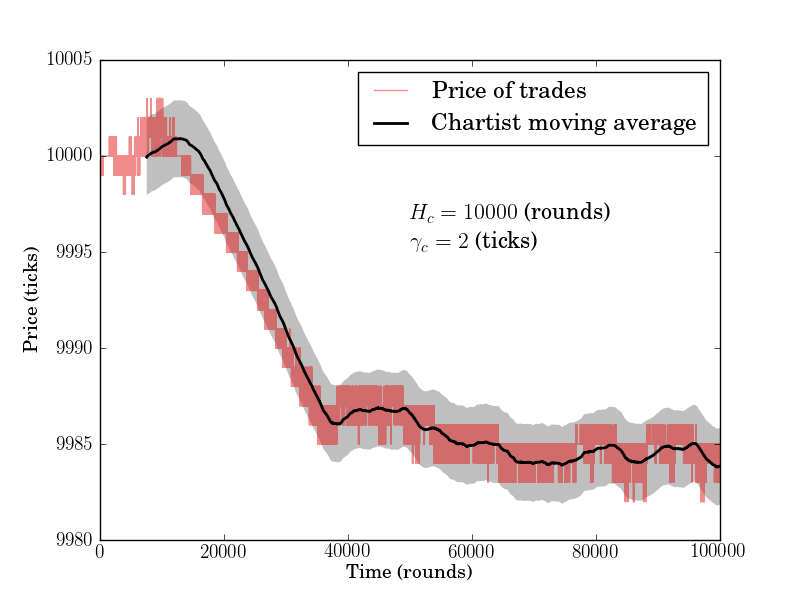
\includegraphics[width=0.5\textwidth]{agent_strategies/marketmaker/d.png}}
\subcaptionbox{}
[0.49\linewidth]{\includegraphics[width=0.5\textwidth]{agent_strategies/marketmaker/b.png}}
\subcaptionbox{}
[0.49\linewidth]{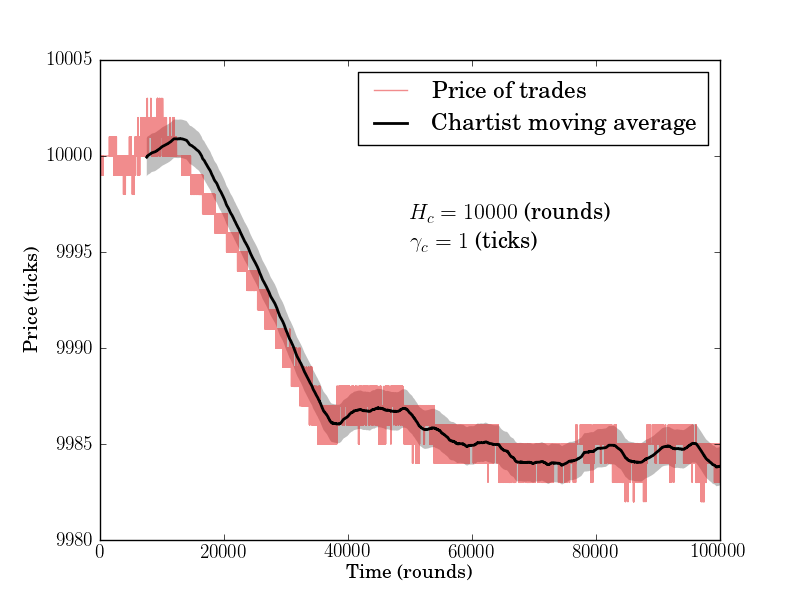
\includegraphics[width=0.5\textwidth]{agent_strategies/marketmaker/c.png}}
\caption{Examples illustrating the how the market maker updates its prices}
\label{figure:marketmaker_strategy}
\end{figure}


\subsubsection{Decision cycle}\label{section_tradeCycles}
Any market maker \marketmaker{i} be thought of as having a trading cycle, the length of which depends on the parameters \ssmmlatencyagent{i} and \ssmmthinkagent{i}. 
\begin{description}
\item[Acquire market information] The agent requests market information at round \round{T_0}. The request reaches the market at round $\round{T_0} + \ssmmlatencyagent{i}$, and the market instantly sends out a reply.
\item[Evaluate market information] The agent receives the market information at round $\round{T_0} +  2\ssmmlatencyagent{i}$, and evaluate its strategy. 
\item[Execute trade decision] The agent reaches a conclusion on how to trade at round $\round{T_0} + 2\ssmmlatencyagent{i} + \ssmmthinkagent{i}$, and sends off an order to the market. The order reaches the market at round $\round{T_0} + 3\ssmmlatencyagent{i} + \ssmmthinkagent{i}$.
\end{description}
As soon as \marketmaker{i} has submitted the new order, it also submits a new request for market information. The agent receives this second batch of market information at round $\round{T_0} + 3\ssmmlatencyagent{i} + \ssmmthinkagent{i}$, and the cycle restarts. The length of the cycle of \marketmaker{i} is therefore defined as
\begin{equation}
\marketmakercyclelength{i} = 3\ssmmlatencyagent{i} + \ssmmthinkagent{i}
\end{equation}
The length of the cycle is important for several reasons. First of all, since the market only requests new market information once during the cycle, the market maker observed the changes in the market with a frequency of $\frac{1}{\marketmakercyclelength{i}}$. Any market events that take place within a period smaller than \marketmakercyclelength{i} can be only partially observed by the market maker.

Secondly, since the market maker can only have a single order on each side of the order book, the latency to the market decides how much volume the market maker is able to buy and sell over a period of time. The market maker $i$ submits orders with a fixed volume \ssmmordervolumeagent{i} and the volume that the agent can supply the market with therefore depends on how much of the time the market maker manages to have standing orders at the market.

When an order submitted by the market maker is filled, the market sends out a transaction receipt which takes \ssmmlatencyagent{i} rounds to reach the market maker. When the market maker receives the receipt, the agent restarts the cycle by submitting a request for market information in order to submit a new order. This means that a total number of $4\ssmmlatencyagent{i} + \ssmmthinkagent{i}$ will elapse from time komma???time that the order was filled to the time when the market maker can have another order placed in the order book. During this time, the market maker does not have an order in the market on the side of the book that the filled order was at. When the market maker does not have a standing order on either side of the book, it means that the agent does not contribute to increasing the liquidity of the asset. Hence, in this simple model, fast market maker should do a better job of supplying liquidity than slow market makers.




%Since it takes $\lambda_n$ rounds for the trade message to reach the market, the total time between the time of the agent requesting market information and the time at which the trade message arrives at the market, is $\round = 3\lambda_n + \lambda_d$. Hence shaving one round of speeds up the entire process of submitting a round by three rounds. 


\subsection{HFT Chartists}\label{section:hft_chartist}
The slow traders do not directly incorporate a chartist element into their strategy, as any changes in the traded price that occurs in the short time that the model simulates would be undetected by the slow traders. However, in order to incorporate chartist behavior in the model, a fast trader agent using a chartist strategy was implemented. These agents will from now on be referred to as HFT chartists, or simply as chartists. 
\subsubsection{Strategy outline}
The chartists use a simple strategy, in which they continually calculate the moving average of the traded prices over a time windows \cite{izumi2009evaluation}. If the current price drops below the moving average, the chartist believes that it has detected a downtrend. The chartists believes that the downtrend will continue for a while, and it will therefore try to get rid of any shares that it is currently holding. In order to accomplish this, the chartists starts to submit sell orders. The more urgently the agent is trying to sell its stocks, the lower it will set the price of the sell order, as a sell order at a lower price is more likely to be filled. On the other hand, if current price rises above the moving average, the agent believes that it has detected an up-trend, and that the stock will be worth more in the near future. The agents therefore starts to submit buy orders starts to submit buy orders at a higher price. The more strongly the agent believes in the stock price increasing, the higher it is willing to set the buy price. The agent only submit orders when it has detected a trend. As long as the chartist does not detect a trend, the agent is inactive and merely observes the market data.  After submitting an order, the agent waits for a while, as a precaution against submitting too many orders which would make the agent incur great losses the trend detected by the agent turns out to be wrong. This mechanism is also a limiting assumption of the model instated in order to protect the market from a few market makers flooding the market with a huge number of orders. As another step towards preventing the order books from filling up with chartist orders that might never be filled, and thus slow down the execution of the simulation, is to make the chartists submit limit orders.

\subsubsection{Parameterization}
The agent strategy is parameterized as follows. HFT chartist agent \chartist{j} has the following parameters:
\begin{description}
\item[Time horizon] The parameter \sctimehorizonagent{j} determines the width of the window over which the agent calculates the moving average. Larger values of \sctimehorizonagent{j} makes the agent use trade price data from further in the past and makes the moving average less responsive to sudden change, while lower values makes the moving average react faster to sudden movements in the price. 
\item[Sensitivity] The sensitivity of \chartist{j} is given by the parameter \scticksbeforereactingagent{j} and refers to the number of ticks that the moving average of the traded price must differ from the currently traded price before the chartist recognizes that it has detected a trend. The higher the value of \scticksbeforereactingagent{j}, the less often the chartist will detect a trend. In the case of $\scticksbeforereactingagent{j} = 0$, the agent will detect a trend whenever $M \neq \currentprice$, which will be true in the majority of rounds.
\item[Aggressiveness] One the chartist decides to trade, it needs to decide upon a price. The aggressiveness parameter \scpriceticksizeagent{j} controls how far from \currentprice that the agent will set the price. This parameter reflects the agents confidence in its own belief about the trend, and the willingness of the agent to trade at sub-optimal prices in order to obtain or sell off shares.
\item[Trading frequency] Once the chartist has detected a trend, it will continue trading for as long as the trend persists. The parameter \scwaitTimeBetweenTradingagent{j} limits the frequency with which the chartist can submitting orders by specifying the number of round that the agent waits before submitting another order.
\end{description}

\subsubsection{Strategy evaluation}
In round \round{T}, the agent calculates the moving average of the buy and sell prices by subtracting the prices that are no longer inside the windows specified by \sctimehorizonagent{}, and adding the the most recent prices. The agent then calculates the average mid-price $\bar{M}_\text{tot}$which is used in the trend detection.
\begin{equation}
\bar{M}_\text{tot} = \frac{1}{2\sctimehorizonagent{}} \bigg[\sum\limits_{n=\round{p}}^{\round{T}} (\bestaskprice{n} + \bestbidprice{n}) - \sum\limits_{n=\round{p} - \sctimehorizonagent{}}^{\round{T} - \sctimehorizonagent{}} (\bestaskprice{n} + \bestbidprice{n})\bigg]
\end{equation}
where \round{p} is the latest round in which the agent was previously active. The agent calculates the current mid-price $m$:
\begin{equation}
m = \frac{\bestaskprice{T} + \bestbidprice{T}}{2}
\end{equation}
The agent then uses a simple rule to decide whether to sell or buy, and at what price:
\begin{flalign}
&\text{Place a buy order if} & & m > \bar{M}_\text{tot} + \scticksbeforereactingagent{} && \text{at buy price} & & p = m + \scpriceticksizeagent{}\\
&\text{Place a sell order if}  & & m < \bar{M}_\text{tot} - \scticksbeforereactingagent{} && \text{at sell price} & & p = m - \scpriceticksizeagent{}
\end{flalign}


Figure \ref{figure:chartist_strategy} provides two examples of how the sensitivity parameter \scticksbeforereactingagent{} and the parameter for the time horizon of the chartist strategy \scticksbeforereactingagent{} influences when the agent will trade or not. In the left figure, the agent has a low sensitivity to price changes, as indicated by the narrow area shaded gray around the black line indicating the moving average calculated by the agent. Since $\scticksbeforereactingagent{} = 1$, the traded price only has to deviate by a single tick from the moving average before the agent will submit orders to trade. In this case, the agent uses a moving average calculated over a relatively short span of $\scticksbeforereactingagent{} = 5000$ rounds, which makes the moving average reflect short-lived price trends. As the figure shows, these parameters prompt the agent to detect trends more or less constantly, and the agent even detects a short up-trend in the beginning of the simulation, as is shown where the traded price (red) does not stay within the gray shaded area . In the right figure, the agent has a sensitivity of $\scticksbeforereactingagent{} = 2$ and a longer time horizon of $\scticksbeforereactingagent{} = 15000$ rounds. Consequently, the agent detects a downtrend in round 12000 or so, where the traded prices, and begins to submit sell orders. However, just before round 40000, the agent decides that the downtrend has ended and the agent becomes inactive until the next time a trend is detected. 
\begin{figure}
%issue 11
\subcaptionbox{\label{subfig:}}
[0.49\linewidth]{\includegraphics[width=0.5\textwidth]{agent_strategies/chartist/a.png}}
\subcaptionbox{\label{subfig:}}
[0.49\linewidth]{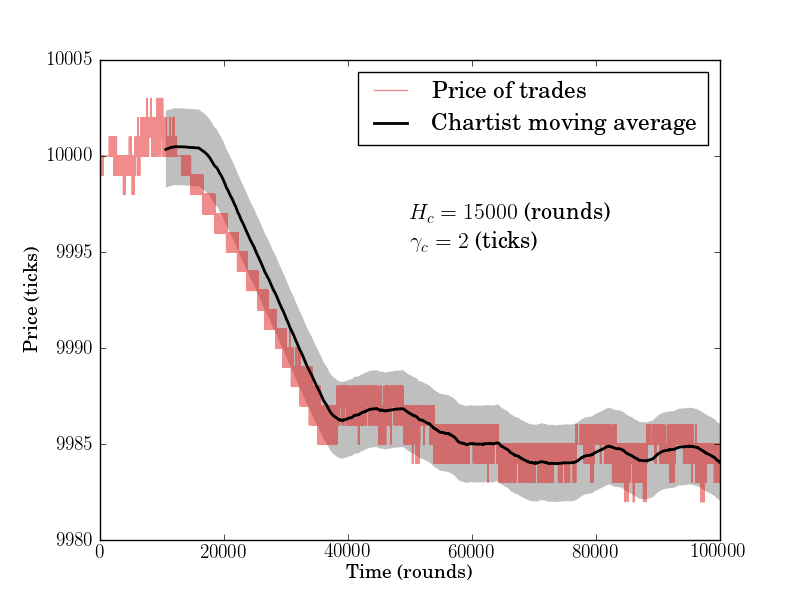
\includegraphics[width=0.5\textwidth]{agent_strategies/chartist/h.png}}
\caption{Examples illustrating the chartist decision strategy}
\label{figure:chartist_strategy}
\end{figure}







%\newpage
%\lhead{\emph{XXX}}
%% Chapter 1

\chapter{Parameter tuning} % Main chapter title

\lhead{Chapter XXX. \emph{XXX}} % This is for the header on each page - perhaps a shortened title
	
%----------------------------------------------------------------------------------------

The model has several parameters which must be selected carefully before the simulation can be used to infer knowledge about market behavior. 

The parameter tuning turned out to consume a significant amount of time, and simple using a genetic algorithm to optimize over the entire space of parameters was not enough. Instead, the process was a slow and iterative one of running the genetic algorithm to create a data set, analyze the data set to find out what was discovered in the search, and then run the genetic algorithm again with different parameters. Thus several data sets were created, each with the purpose of examining some aspect of the simulation, or of the parameter tuning method itself. 

This chapter will cover the instruments used in the optimization of the model parameters, and also mention the machine learning tools used in the analysis of the data sets. 

The parameter tuning has two overall goals, which are covered in the following section.

\section{Motivation and overall procedure}
First of all, the model must be calibrated such that it mimics the behavior of real markets. Since virtually every aspect of the simulation behavior depends on the values on the various parameters, these must be chosen carefully in order for the simulation to produce realistic behavior. An example of a simulation untuned parameters causing  unrealistic behavior is given in figure \ref{subfig:unrealistic_behavior}. Selecting realistic parameters is by far a simple task. First of all, it requires a way of quantifying the quality of each simulation. The choice of such a quantification is discussed in section \ref{section:simulation_fitness}. Secondly, there might be several different parameter configurations which produce seemingly realistic behavior, but do not correspond to a realistic market setting. An example for this is given in figure \ref{subfig:unrealistic_parameters}, and section \ref{section:filtering_parameters} briefly discusses this point. 

\begin{figure}
	%issue 15
	\subcaptionbox{Parameters causing unrealistic dynamics\label{subfig:unrealistic_behavior}}
	[0.49\linewidth]{
\includegraphics[width=0.5\textwidth]{Electron.pdf}}
	\subcaptionbox{Unrealistic parameters causing realistic dynamics\label{subfig:unrealistic_parameters}}
	[0.49\linewidth]{
\includegraphics[width=0.5\textwidth]{Electron.pdf}}
	\caption{\textbf{Motivatoin for tuning:} the two}\label{fig:tuning_motivation}
\end{figure}

The second goal of the parameter tuning is to find parameters which promotes certain desirable behaviors. For instance, we might be interested in determining which parameters causes the traded price to stabilize faster after a shock to the fundamental price. Metrics for doing this is discussed in section \ref{section:simulation_fitness}

The selection of parameters is a fairly complicated process because of the large parameter space, and because it takes a significant time to evaluate the fitness of a given set of parameters\footnote{The calculation time depends largely on the parameters, such as the number of agents and how active these are. Typically one to several minutes are required to evaluate a single set of parameters.}. amount of time to execute a simulation. Because of this, the following three-step parameter selection procedure was used.
\begin{enumerate}
	\item Fix some of the model parameters in order to reduce the search space for the optimization algorithm. This requires us to consider which parameters can be fixed without losing opportunity to gain insight into market behavior. Essentially this step is a question of prioritizing the optimization of some parameters over the optimization of others. 
	\item Use an optimization algorithm to find sets of parameters which yield realistic model behavior. A genetic algorithm was chosen for this purpose, and the details are explained in section \ref{section:genetic_algorithm}.
	\item From the set of parameter combinations found by the optimization algorithm, remove the parameter combinations which obviously do not correspond to a realistic setting.
\end{enumerate}

\subsection{Selecting fixed parameters}
The main parameters of interest are the ones that control the latency and speed of the agents. The agent strategy parameters are less important, since 



\begin{description}
	%issue 16
	\item [\nrounds] Due to the computational cost of running the simulation for a large number of rounds, the the number of rounds is fixed at $10^5$ for all experiments.
	\item [Order volumes] As with most of the other agent parameters, the 
\end{description}

The remaining model parameters will either be fixed for each experiment, or varied by the genetic algorithm. 





\section{Inverse simulation with a genetic algorithm}\label{section:genetic_algorithm}
%issue 5
Inverse simulation refers to the technique of specifying metrics measuring model behavior, and then using an optimization algorithm to search for parameters resulting in desirable (or undesirable) behavior. 

In this work, a genetic algorithm was used to search the parameter space. The algorithm proceeds as explained below.
\begin{enumerate}
	\item Generate a population of healthy individuals, e.g., individuals with valid parameters.
	\item Evaluate fitness for every individual in the population.
	\item Repeat $n_\text{gen}$ times 
	\begin{enumerate}
		\item Generate offspring by crossing existing individuals.
		\item Apply mutation to with a certain probability to each individual (parents as well as children)
		\item Evaluate fitness of children and mutated parents.
	\end{enumerate}
\end{enumerate}

Mutation and crossover are the operators responsible for generating variation in the population, while the selection is responsible for propagating promising individuals to future generation where they might be improved. Several possible methods of performing each of these three steps exist in the literature (see\cite{genetic1}, \cite{genetic2}), and section \ref{section:ga_parameters} briefly covers the method and parameters of the genetic algorithm.

\subsection{Representing parameters as genes}
Since the choice of mutation and crossover operators depends on the nature of the genes, the first step towards utilizing to search the model parameters is to decide on how to encode the parameters as individuals. 
A set of parameters is represented by an individual, $i$, consisting gene for each parameter, represented by a floating point $g_{i,j}$, where $j$ denotes the index of the parameter. When the population is initialized, each $g_{i,j}$ is drawn from a uniform distributed in the range $g_j \in [0;1]$:
\begin{equation}
g_{i,j} \sim \mathcal{U}(0,1)
\end{equation}


Some of the model parameters are integers, such as \nmm and \nsc, and these are rounded after being scaled and before they are passed to the simulation.



%issue 17


\subsection{Model fitness}\label{section:simulation_fitness}

In order to use inverse simulation, it is necessary to decide on how to measure the quality of an instance of the simulation. In this work, the overall goal is to examine which parameter values cause the market to be stable, and which cause it to be unstable. 


Another interesting point is the speed with which the market responds to the shock to the fundamental price, and which parameters influence this property. Furthermore, we are interested in investigating whether or not 

\begin{itemize}
\item 'fit
\item Are there certain parameter combinations which cause the market to behave in certain ways. S
\end{itemize}
In particular the parameters controlling various time delays are of interest. 
The search space of the parameters is very large, which makes an exhaustive search impossible.
To this end, four fitness measures were defined.
The balance between the number 
Several parameters influence the number of orders submitted by the high frequency traders.

\subsection{Genetic algorithm parameters}\label{section:ga_parameters}
Although this is a basic version of genetic algorithm, using it correctly is not necessarily easy, as was encountered. First of all, the parameters for the genetic algorithm itself must be established. The larger and more complex the search space, the more resources the search will require, since the evaluating the fitness function (i.e., the running the simulation) will have to be done a larger number of times. 



Table \ref{table:genetic_algorithm_parameters} presents an overview of the parameters used in the genetic algorithm. 

\begin{table}
	\centering
	\begin{tabular}{l|l}
		Parameter & Assignment\\\hline
		Number of generations & 200 to 1000\\
		Number of individuals & 100 to 1000\\
		Cross-over points & 2\\
		Tournament size & 3\\
		Mutation probability & 0.1\\
		Mutation distribution &  $\mathcal{N}(\mu = 0, \sigma = 0.1)$\\
	\end{tabular}
	\caption{Overview of parameters used in the genetic algorithm}
	\label{table:genetic_algorithm_parameters}
\end{table}


\subsection{Controlling market behavior}
The four fitness measures defined in section \ref{section:simulation_fitness} make it possible to specify the type of market behaviour that is favoured by the genetic algorithm. gives 16 combinatinos for how to optimize the model. 

First of all, we are interested in establishing which parameters cause the market to return to a stable state after the fundamental price has incurred a shock

\begin{table}
\begin{tabular}{c|c}
\textbf{Parameter} & \textbf{Range}\\
\nmm & \\
\nsc & 
\end{tabular}
\caption{Overview of experiments}
\label{table:optimization_goals}
\end{table}


\subsection{Filtering parameters}\label{section:filtering_parameters}
As mentioned earlier, it is not enough simply to define a fitness function which assigns high values to parameters causing realistic behavior. In addition, it is important to discard parameters which obviously do not correspond to a realistic setting. Imagine that the simulation scores high fitness values when executed without any market makers. Since it is known that real markets do in fact contain market makers, nothing can be inferred from such a result. Indeed this might be a consequence of poorly designed fitness measures, but since it is easier to use domain specific knowledge to filter out the unrealistic parameters

\begin{figure}[htbp]
	\centering
		
\includegraphics{Figures/Electron.pdf}
		\rule{35em}{0.5pt}
	\caption{Example of a simulation which is assigned fairly good fitness values, but which was executed with clearly unrealistic parameters: $\nmm = \nsc = 0$. The simulation reaches the new fundamental price fairly quickly without any undershoot, and stays within the stability margin. The only point where it scores badly is the standard deviation which is slightly high due to the fluctuating trade price.}
	\label{fig:no_marketmakers}
\end{figure}


\subsection{Handling failed simulations}\label{section:failed_simulations}
\begin{figure}\subcaptionbox{\ssmmlatencymu=49, \ssmmlatencys=8, \sclatencymu=32, \sclatencys=19, \overshoot=1.0, \timetoreachnewfundamental=29210.0, \roundstable=23970.0, \stdev=0.482\label{no_reaction_0}}[0.49\linewidth]{\includegraphics[width=0.5\textwidth]{/Users/halfdan/Dropbox/Waseda/Research/MarketSimulation/Thesis/data_for_figures/test/gen0_1387987146731556L.png}}
\subcaptionbox{\ssmmlatencymu=7, \ssmmlatencys=17, \sclatencymu=21, \sclatencys=17, \overshoot=1.0, \timetoreachnewfundamental=28229.0, \roundstable=23146.0, \stdev=0.5\label{no_reaction_1}}[0.49\linewidth]{\includegraphics[width=0.5\textwidth]{/Users/halfdan/Dropbox/Waseda/Research/MarketSimulation/Thesis/data_for_figures/test/gen0_1387987146764027L.png}} \end{figure}

Some parameters cause the simulation to act in strange ways, and even crash in some cases. For instance, the the order book becomes empty, the simulation throws an exception and terminates. Similarly, if the best \bid/\ask prices drops to zero, the simulation exits. As such 

The most common odd phenomenon was the market 


\section{Applying the genetic algorithm}
Applying the genetic algorithm to produce markets with desirable behavior turned out to be more difficult that one could have hoped for. First of all, the high computational costs was a hurdle. 

Secondly, many of the data sets (see section \ref{section:gene_pool_as_data_set}) produced did not contain any useful information. 

The model parameters do influence the fitness values as they control model behavior, but they are not directly weighted into the fitness-values. This means that even after the parameters of the genetic algorithm was properly tuned in such a way that higher-fitness individuals were produced, these individuals often turned out to be of no interest. Such individuals were discarded according to the filtering criteria described in section \ref{section:filtering_parameters} would have to be discarded. An example of such a case is discussed in section \ref{}

\subsection{Time complexity}
The high time complexity stems from several factors
\begin{itemize}
\item Running a simulation for a given set of parameters required up to several minutes of computation on a single CPU core.
\item Large number of model parameters increase the size of the search space. The more parameters Unfortunately there is no magic to the way the genetic algorithm works, and optimizing in a larger search means a larger time complexity.
\item Large range of parameters. Some of the parameters are integers while some are real numbers. While most of the parameters have a lower bound, none of the parameters have upper bounds.
\item Unstable fitness parameters. Since the same set of parameters can produce varying model behavior, the fitness-values may also vary. Therefore it is necessary to evaluate the simulation several times for each set of parameters. 
\item The model parameters also influence the time complexity. For instance, evaluating a simulation with many agents takes more time than evaluating a simulation with fewer agents. 
\end{itemize}

Genetic algorithms are naturally suited for parallel computation. Two servers with a total of 40 cores and enough memory to evaluate as many simulations were utilized. With this equipment, evaluating a single strategy (see section \ref{section:datasets_introduction})for generating data sets could take 

reaching a point where the genetic algorithm began to produce useful output turned out to be somewhat of an iterative process. 


First of all, the computational cost of running the genetic algorithm was high, which meant that the algorithm was not always able to find better individuals. 

Det tager lang tid -> faerre params
skod resultater -> nye experimenter


Second of all, even when the genetic algorithm did manage to improve the fitness of the population, this did not always result in useful data. 

\subsection{Experiments: Dividing the search into parts}\label{section:datasets_introduction}
As mentioned earlier, the number of parameters and the range of each parameter influences the complexity of the search. Because of this, it is desirable to keep the number of parameters that are included in each individual as small as possible. However, fixing parameters means that some interesting properties about the model might not be discovered. Furthermore, varying all parameters at the same time makes the analysis and interpretation of the results more difficult. In an attempt to overcome this dilemma, several ``experiments'' were carried out \footnote{The reason for the quotes is that the term experiment might be stretching the common understanding of what an experiment is a little.}. Instead of trying to optimize all the model parameters at once, the search was split into several parts, each of which we call an experiment. Each of these experiments produce a data set, each of which were analyzed using the methods described in section \ref{section:data_analysis_techniques}. Some of the data sets produced interesting results, while others did not. Chapter \ref{chapter:results_and_discussion} focuses on the analysis and presents the findings. A brief overview of the experiments is presented in \ref{section:experiments_overview}, but since the motivation for creating each data set is best understood in the context of the analysis of each data set, the details are deferred until chapter \ref{results_and_discussion}. The next section will explain exactly what a data set is.

\subsection{Gene pool as data set}\label{section:gene_pool_as_data_set}
The previous sections contain the details of each of the steps undertaken in order to produce data sets. To summarize, the list below enumerates the steps.
\begin{enumerate}
\item Initialize a population in the genetic algorithm with healthy individuals.
\item Evaluate the fitness for every individual several times and obtain fitness-values by calculating averages.
\item Stack all individuals that ever lived into a $\datasetNpoints \times \individuallength$ parameter data matrix \datamatrixpar, where $\datasetNpoints$ is the number of individuals, and $\individuallength$ is the length of each individual. Likewise, stack the fitness values into a $\datasetNpoints \times \fitnesslength$ fitness-data matrix \datamatrixfit, where \fitnesslength is the number of fitness values calculated. 
\item Filter the data by removing rows in \datamatrixpar with parameters which can be deemed not to correspond to real markets, and by removing rows in \datamatrixfit with fitness values that are not realistic. Please refer to section \ref{section:filtering_parameters} for details. Naturally, when a row is removed in \datamatrixpar, it is also removed in \datamatrixfit, and vice versa. 
\item Likewise, data points which were generated by a simulation crashing before it could complete were removed.
\end{enumerate}
Tables \ref{table:example_dataset_parameters} and \ref{table:example_dataset_fitnesses} contain the first rows of \datamatrixpar and \datamatrixfit for one of the data sets.
\begin{table}
\centering
\scriptsize
\begin{tabular}{lrrrrrrrrrrrrrr}
\toprule
{} &  \sclatencymu &   \sclatencys &   \scnAgents &   \scthinkmu &   \scthinks &   \sctimehorizonmu &   \sctimehorizons &   \scwaitTimeBetweenTradingmu &   \scwaitTimeBetweenTradings &   \ssmmlatencymu &   \ssmmlatencys &   \ssmmnAgents &   \ssmmthinkmu &   \ssmmthinks \\
\midrule
0 &            84 &            11 &           14 &           98 &           9 &               1071 &               445 &                            38 &                           17 &                3 &               2 &             48 &              8 &             1 \\
1 &            23 &            21 &           74 &           49 &          24 &                529 &               554 &                            45 &                           13 &                9 &               0 &              8 &              5 &             3 \\
2 &            51 &            13 &           53 &           47 &          13 &               3586 &               536 &                            10 &                           11 &                9 &               4 &             14 &              4 &             2 \\
3 &            18 &            21 &          213 &           70 &          39 &                793 &              1179 &                            33 &                           15 &                7 &               2 &             43 &              6 &             3 \\
4 &            94 &            41 &          144 &           10 &          25 &               2668 &               893 &                            12 &                           15 &                6 &               1 &             49 &              7 &             4 \\
5 &            19 &             4 &          130 &           15 &          38 &               1085 &              1165 &                            39 &                            4 &                2 &               3 &             11 &              4 &             4 \\
6 &            65 &            15 &           91 &           81 &          46 &               3867 &              1991 &                            48 &                            1 &                7 &               2 &             21 &              4 &             4 \\
7 &            36 &            38 &          143 &           77 &          19 &               2805 &              1870 &                            10 &                            9 &                7 &               0 &              3 &              2 &             4 \\
8 &            43 &             8 &           10 &           19 &          19 &               3384 &              1706 &                            33 &                            4 &                8 &               4 &              5 &              5 &             0 \\
9 &            11 &            33 &          127 &           94 &          49 &               3597 &               723 &                            12 &                            2 &                7 &               1 &             33 &              5 &             4 \\
\bottomrule
\end{tabular}

\caption{An example data matrix containing the parameters of ten individuals who lived sometime during the execution of the genetic algorithm. In this case, each individual contained parameters for the number of HFT agents, as well as the latency and thinking time parameters. Hence, the data matrix has a column for each parameter.}
\label{table:example_dataset_parameters}
\end{table}

\begin{table}
\centering
\begin{tabular}{lrrrr}
\toprule
{} &  \overshoot &   \roundstable &    \stdev &   \timetoreachnewfundamental \\
\midrule
0 &           3 &          25359 &  0.382092 &                        29838 \\
1 &           7 &          99999 &  1.289659 &                        23373 \\
2 &           6 &          99999 &  1.253363 &                        18748 \\
3 &           7 &          99997 &  1.695150 &                        22819 \\
4 &           6 &          94343 &  1.329276 &                        22703 \\
5 &          16 &          99999 &  2.439084 &                        31860 \\
6 &           6 &          93378 &  1.287235 &                        25645 \\
7 &          10 &          99997 &  1.858166 &                        19417 \\
8 &           3 &          24039 &  0.935465 &                        27381 \\
9 &          19 &          99995 &  4.092439 &                        24845 \\
\bottomrule
\end{tabular}

\caption{This table contains the fitness values for each individual in table \ref{table:example_dataset_parameters}. Note that, in order to increase the reliability of the fitness measure of an individual, the recorded fitness-values are the average of the fitness-values obtained by evaluating each individual ten times}
\label{table:example_dataset_fitnesses}
\end{table}

\subsection{Convergence of parameters}

\section{Data analysis tools}\label{section:data_analysis_techniques}
Using inverse simulation merely creates a lot of data. This data has to be analyzed before any 

Data normalization

\subsection{Data visualization}
It is useful to be able to plot the data points 

\subsubsection{Color toned scatter plots}
Scatter plots are useful for initial data analysis, as one can quickly detect problems such as outliers, and maybe even detect clusters of data points. 

\subsection{Preprocessing}

\subsubsection{Handling outliers}
The term outliers is often used as a label for data which is considered ``invalid'' in the sense that is not a product of the true data generation process, but  due to various sources of noise. In this report, data that was caused by failing simulations corresponds to the usual understanding of outliers. However, as was already explained in section \ref{section:failed_simulations}, data from such simulations are never included in \datamatrixpar{} and \datamatrixfit{} to begin with. Instead, outliers in this report refer to entries in \datamatrixpar{} and \datamatrixfit{}  deviate significantly from the majority of the data points by having extreme values.

Such data points caused problems when applying data analysis techniques which rely on a fairly normal distribution of the data points, such as Principal Component Analysis (PCA). PCA looks for a rotation of the data space, such that the axes of the new basis are aligned with the directions of the largest variance in the original space. Since a few points with extreme values come to account for a large portion of the data set variance, the new basis computed by PCA will be aligned along these few data points. When PCA is used to extract lower dimensional features from the data set, outliers will degrade the quality of these features. In the case that PCA is used for data visualization, the scatter plots of the first few principal components will not be very informative, as they merely show the projection of the data onto the axes aligned with the outliers.

In all experiments, outliers were present in both the parameters space and in the fitness space. Outliers in the parameter space occur because of abnormally large mutations, and any dimension of the parameter space is susceptible to such an event. In the fitness space, only a few of the features suffered from the occurrence of outliers. The feature \roundstable cannot contain outliers, because the shock to the fundamental occurs at round $\round = 10^4$, and because the simulation is terminated at round $\round = 10^5$, hence $\roundstable \in [10^4,10^4+1,\hdots 10^5]$. The same is true for \timetoreachnewfundamental. \stdev and \overshoot, on the other hand, are susceptible to outliers, because the two features have no upper bound.


\begin{enumerate}
\item Apply a monotonically increasing transformation $f(x)$ to some or all of the features for every data point in the data set. A common choice of $f$ is $f(x) = \log x$, as it efficiently reduces the impact of data points with extremely high values. Figure \ref{figure:scatter_log_transform} illustrates the effect of applying the log-transform. The log-scaling does a fairly good job of reducing the importance of the outliers in the \stdev feature, while the change is less dramatic in \timetoreachnewfundamental. While the left scatter plot does not really reveal any structure of the data, the transformation makes it possible to spot to rough clusters when inspecting the right plot.

Another simple method is to manually remove 
\item Manually select one or more criteria for when a data point is to be considered an outlier. It is worth noticing that \overshoot and \stdev 
\item Use a one-class support vector machine to calculate a probability for each data point that said point is an inlier or an outlier. In this case, inliers 
\end{enumerate}

\begin{figure}\label{figure:scatter_log_transform}
\subcaptionbox{Untouched data}
[0.49\linewidth]{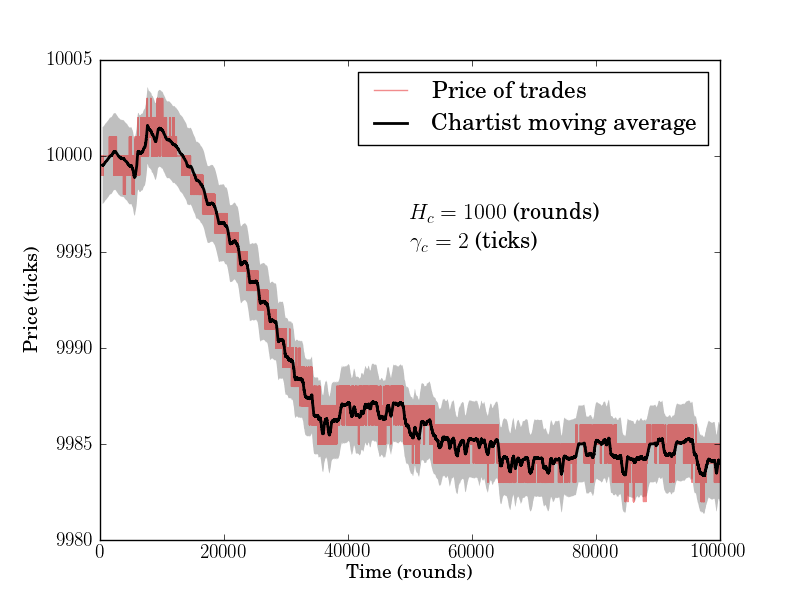
\includegraphics[width=0.5\textwidth]{21_scatter_plots/d3/f.png}}
\subcaptionbox{Log-scaled}
[0.49\linewidth]{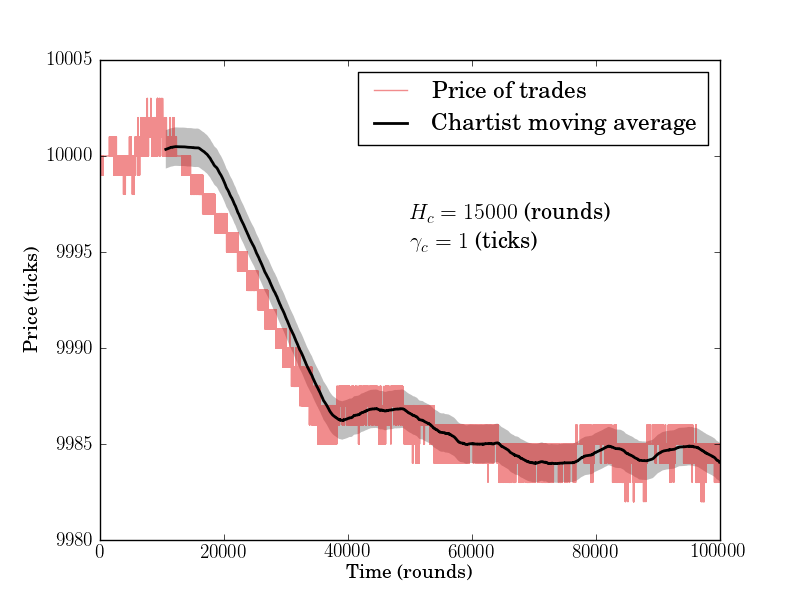
\includegraphics[width=0.5\textwidth]{21_scatter_plots/d3/g.png}}
\subcaptionbox{Outliers manually removed}
[0.49\linewidth]{\includegraphics[width=0.5\textwidth]{103_scatter_manual_outlier/d3/a.png}}
\subcaptionbox{Log-scaled and without outliers}
[0.49\linewidth]{\includegraphics[width=0.5\textwidth]{103_scatter_manual_outlier/d3/b.png}}
\caption{Color toned scatter plots of \timetoreachnewfundamental, \stdev and \roundstable taken from dataset \dthree after applying log-scaling and manually removing outliers}
\end{figure}


In the parameters data set, outliers can occur due to abnormally large mutations. 
Some parameters cause the simulation to act in strange ways, and even crash in some cases. For instance, the the order book becomes empty, the simulation throws an exception and terminates. Similarly, if the best \bid/\ask prices drops to zero, the simulation exits. As such 

The most common odd phenomenon was the market 



\subsubsection{title}
\subsection{Clustering algorithms}


\newpage
\lhead{\emph{XXX}}
\part{Experiments}\label{chapter:experiments_and_results}
As mentioned in the previous chapter, the process of finding was an iterative one of running an experiment, analyzing the generated data, draw conclusions and then repeat the steps with a new experiments designed to amend the mistakes of the previous experiment. This chapter will go through the results that were obtained from each of the data sets. A summary and discussion of the results is found in chapter \ref{chapter:discussion}.

\section{Overview of experiments}
The model has many parameters, and doing an exhaustive search over the entire parameter space is not possible. Instead, a genetic algorithm (GA) was used to do targeted searches of the parameters. For the details of the GA, please see chapter \ref{chapter:ga}. Depending on how the GA was set up, different areas of the search space was searched. Even when using a GA, some parameters had to be fixed. However, fixing parameters means that the effect of the fixed parameter on the behavior of the model remains unknown, since only a subspace of the entire parameter space is searched. For this reason the genetic algorithm was executed several times, each creating a data set containing fitness values for different parts of the parameter space. Each of these data set can be analyzed, providing information which can be corroborated in order to form an understanding of the overall market behavior.

Table \ref{table:datasets_overview} contains an overview of the different data sets, showing which parameters were fixed, and which were included as genes in the genetic algorithm.

In the following four experiments, the genetic algorithm was set to minimize all four fitness-measures.

\begin{description}
\item[\dthree: Varying the number of HFT agents, and all latency related parameters] This data set was generated by including all the model parameters concerning time latency as well as the number of agents into the individuals in the genetic algorithm. Due to the high number of variables, the data turned out to be difficult to analyze, as too many factors pertaining to the simultaneous change of several parameters influenced the fitness values.
\item[\dnine: Fixing the number of agents while varying latency parameters] The analysis of \dthree{} showed that when minimizing the four fitness-measures, the genetic algorithm tended to select  model containing few or no HFT agents. The case of a market with no market makers and no chartists can safely be said to be trivial. Hence, in experiment \dnine, the number of HFT agents were fixed to $\ssmmnAgents = 30$ and $\scnAgents = 100$.
\item[\dten: Fixing the number of HFT chartists] Since \dnine kept \ssmmnAgents and \scnAgents constant, the experiment did not reveal anything on how the market behavior changes when the number of agents changes. In order to investigate the impact of having many or few HFT market makers, \ssmmnAgents was varied in this experiment. Although it is also of interest how the market behavior depends on the number of HFT chartists, including \scnAgents as a gene would yield results similar to those obtained in \dthree. For this reason the number of HFT chartists was fixed to $\scnAgents = 150$.
\item[\deleven: Fixing the number of HFT market makers] This experiment was carried out in order to investigate the impact of the number of HFT chartists on the market behavior, and is supplementary to \dten.
\end{description}


\begin{table}
\begin{tabular}{|l|L|E|L|}
\toprule
ID & Description & Fixed parameters& As genes \\
\midrule
\dthree & All parameters varied& $\scordervolumemu=10$,$\scordervolumes=3$,$\ssmmordervolumemu=50$,$\ssmmordervolumes=20$,$\scticksbeforereactingmu=2$,$\scticksbeforereactings=5$,$\scpriceticksizemu=3$,$\scpriceticksizes=2$ &  \sclatencymu, \sclatencys, \scnAgents, \scthinkmu, \scthinks, \sctimehorizonmu, \sctimehorizons, \scwaitTimeBetweenTradingmu, \scwaitTimeBetweenTradings, \ssmmlatencymu, \ssmmlatencys, \ssmmnAgents, \ssmmthinkmu, \ssmmthinks\\
\midrule
\dnine & Fixed number of HFT agents &$\ssmmnAgents = 30$, $\scnAgents = 100$,$\scordervolumemu=10$,$\scordervolumes=3$,$\ssmmordervolumemu=50$,$\ssmmordervolumes=20$,$\scticksbeforereactingmu=2$,$\scticksbeforereactings=5$,$\scpriceticksizemu=3$, $\scpriceticksizes=2$ & \scthinkmu, \scthinks, \sctimehorizonmu, \sctimehorizons, \scwaitTimeBetweenTradingmu, \scwaitTimeBetweenTradings, \ssmmlatencymu, \ssmmlatencys, \ssmmnAgents, \ssmmthinkmu, \ssmmthinks \\
\midrule
\dten & Fixed number of HFT chartists and fixed strategy parameters & $\scnAgents = 150$, $\ssmmthinkmu = \scthinkmu = 50$, $\ssmmthinks = \scthinks = 20$, $\sctimehorizonmu = 5000$, $\sctimehorizons = 2000$, $\scwaitTimeBetweenTradingmu = 50$, $\scwaitTimeBetweenTradings = 20$,$\scordervolumemu=10$,$\scordervolumes=3$,$\ssmmordervolumemu=50$,$\ssmmordervolumes=20$,$\scticksbeforereactingmu=2$,$\scticksbeforereactings=5$, $\scpriceticksizemu=3$,$\scpriceticksizes=2$  & \ssmmnAgents, \sclatencymu, \sclatencys, \ssmmlatencymu, \ssmmlatencys \\
\midrule
\deleven & Fixed number of HFT market makers and fixed strategy parameters & $\ssmmnAgents = 52$, $\ssmmthinkmu = \scthinkmu = 50$, $\ssmmthinks = \scthinks = 20$, $\sctimehorizonmu = 5000$, $\sctimehorizons = 2000$, $\scwaitTimeBetweenTradingmu = 50$, $\scwaitTimeBetweenTradings = 20$,$\scordervolumemu=10$,$\scordervolumes=3$,$\ssmmordervolumemu=50$,$\ssmmordervolumes=20$,$\scticksbeforereactingmu=2$,$\scticksbeforereactings=5$, $\scpriceticksizemu=3$,$\scpriceticksizes=2$  & \ssmmnAgents, \sclatencymu, \sclatencys, \ssmmlatencymu, \ssmmlatencys \\
\bottomrule
\end{tabular}
\caption{Overview of datasets}
\label{table:datasets_overview}
\end{table}


\subsection{Correlation between fitness measures}\label{section:correlation_fitness}
A factor which influences the evolution of parameters is correlation between the fitness-measures. If two or more fitness measures have non-negative correlation coefficients, individuals will be statistically more likely to get good scores in the correlated fitness measures at the same time. Since all fitness measures are given equal weight in the selection process, individuals scoring well in the correlated fitness-measures will win over individuals which score well on another, statistically independent fitness measure. It is therefore important to compare the selection tendencies with the correlation between fitness-measures. Figure \ref{figure:d10_fitness_correlation} shows a plot of the correlation matrix for \dten. Since later generations will be affected by the biased selection and therefore contain more individuals which did well on the correlated fitness measures, the correlation coefficients in the figure were calculated over individuals in the first generation only.
\begin{figure}
\centering

\includegraphics[width=0.7\textwidth]{Electron.pdf}
\caption{Correlation matrix of the four fitness measures in the first generation of dataset \dten	}
\label{figure:d10_fitness_correlation}
\end{figure}

For instance, the correlation between \overshoot and \stdev means that an individual which scores a good \overshoot-fitness will be statistically likely to also score a good \stdev-fitness. Since all four fitness measures are weighed evenly in the selection, models with behavior which is assigned good values for \overshoot and \stdev will score a better overall fitness than a simulation with a good fitness 

In other words, the correlation between \stdev and \overshoot means that stable individuals will outlive fast individuals as they are selected for breeding more often. This is not a property of a model itself, but rather a problem with the definition of the fitness measures. This problem can be circumvented by not using of the correlated fitness values. XXX

Both \overshoot and \stdev were used for the GA selection, and although these two fitness measures do reflect different properties of the simulations, they were found to be somewhat correlated. That is, a simulation which tends to have a small overshoot also tends to have stable traded prices. 

 (simulations with a small overshoot also tend to have more stable trade prices), and there work together towards selecting the same type of simulations. \timetoreachnewfundamental and \roundstable both  The same is not the case for \timetoreachnewfundamental and \roundstable, as it possible that a simulation responds quickly to the shock, but does not stay within the stability margin. 

\section{Fitness and parameter evolution}\label{section:fitness_and_paraeter_evolution}


\subsection{Variable number of market makers}

Figure \ref{fig:d10_evolution_fitness} shows the evolution of the four fitness measures. The population wide mean is plotted along the median and minimum statistics. Since all four fitness measures were minimized, the curve for the minimum value shows the best individual alive during each generation, with respect to each fitness measure. While the mean reflects how the overall population is evolving,  the median is useful as it gives an insight into how skewed the population wide distribution of parameters is. 


\begin{figure}
	%issue 15
	\centering
	\subcaptionbox{Evolution of \roundstable\label{fig:d10_evolution_fitness_a}}
	[0.49\linewidth]{\includegraphics[width=0.5\textwidth]{82_generation_plots/d10/round_stable.png}}
	\subcaptionbox{Evolution of \timetoreachnewfundamental\label{fig:d10_evolution_fitness_b}}
	[0.49\linewidth]{\includegraphics[width=0.5\textwidth]{82_generation_plots/d10/time_to_reach_new_fundamental.png}}
	\subcaptionbox{Evolution of \stdev\label{fig:d10_evolution_fitness_c}}
	[0.49\linewidth]{\includegraphics[width=0.5\textwidth]{82_generation_plots/d10/stdev.png}}
	\subcaptionbox{Evolution of \overshoot\label{fig:d10_evolution_fitness_d}}
	[0.49\linewidth]{\includegraphics[width=0.5\textwidth]{82_generation_plots/d10/overshoot.png}}
	\caption{Evolution of the four fitness measures in experiment \dten}
	\label{fig:d10_evolution_fitness}
\end{figure}





\begin{description}
\item[Model stability]
Figure \ref{fig:d10_evolution_fitness_a}: shows that  the GA quickly manages to find some parameters which cause the simulation to stabilize quickly. However, these individuals do not manage to dominate the population evident by the mean and median curves remaining almost the same until generation 30 or so. In the next 20 generations the population undergoes a rapid change, as the population wide average of \roundstable drop from close to $10^5$ to around $2\cdot 10^4$ rounds on average. The disparity between the mean and the median indicates that the population undergoes a rapid change in the same period, from mostly containing unstable individuals to mostly containing stable individuals. In generation 42, the median curve crosses the mean curve, which means that the the population contain as many stable simulations as it contain unstable simulations. From that point on the unstable simulations are quickly replaced by stable individuals.
\item[Price fluctuations and overshoot]
During the same period, the population average \stdev also decreases fairly rapidly, but the drop is less pronounced than the drop in \stdev. As figures \ref{fig:d10_evolution_parameters_a} and \ref{fig:d10_evolution_parameters_b} show, the number of market makers rapidly increased during this period, as did the average latency of the market makers. Since the mean and median are close in both figure\footnote{Since \overshoot is discrete, the median and $\min$ statistics are also discrete}, the mean is representative of the evolution of the entire population.
\item[Responsiveness]
\timetoreachnewfundamental measures the time it takes for the model to react to the shock in the fundamental, and the evolution of the population wide statistics is shown on figure \ref{fig:d10_evolution_fitness_b}. Although the GA is instructed to minimize \timetoreachnewfundamental in order to look for more faster models, it clearly fails to do this. Indeed, the most responsive simulation took only about 4000 rounds to reach the new fundamental, but this individual died out in favor of slower individuals. In the last generation the most responsive simulation took around 14000 rounds to reach the new fundamental. The reasons for this failure to locate responsive models is discussed in section \ref{section:correlation_fitness}. In the A large change of the average of \timetoreachnewfundamental happens in the rounds five to 15. In this period, the median is lower than the mean, which means that the growth in the mean can be attributed to a minority of individuals.
\end{description}


On figures \ref{fig:d10_evolution_fitness} and \ref{fig:d10_evolution_parameters}, the two areas shaded in a light blue and light red respectively show the two periods during which there was a drastic change in parameters and fitness-values. By comparing the time at which parameters and fitness-values change, it is possible to get an idea of how parameters influence the fitness-values. To that end, figure \ref{fig:d10_evolution_parameters} shows the evolution of each of the parameters that were varied by the GA\footnote{Since the median was found to follow the mean nicely for all the parameters, the medians are not displayed. Also, the gray error bars show the population wide variance}.
\begin{figure}
	%issue 15
	\centering
	\subcaptionbox{Evolution of \ssmmlatencymu{} and \sclatencymu\label{fig:d10_evolution_parameters_a}}
	[0.49\linewidth]{\includegraphics[width=0.5\textwidth]{82_generation_plots/d10/latpars_mu.png}}
	\subcaptionbox{Evolution of \ssmmlatencys{} and \sclatencys\label{fig:d10_evolution_parameters_b}}
	[0.49\linewidth]{\includegraphics[width=0.5\textwidth]{82_generation_plots/d10/latpars_s.png}}
	\subcaptionbox{Evolution of \ssmmnAgents\label{fig:d10_evolution_parameters_c}}
	[0.49\linewidth]{\includegraphics[width=0.5\textwidth]{82_generation_plots/d10/nAgents.png}}
	\caption{Evolution of the model parameters in experiment \dten}
	\label{fig:d10_evolution_parameters}
\end{figure}

The two periods indicated by the shaded squares seem to reflect some sudden changes in the parameters.

\begin{description}
\item[Average agent latency]  As is shown on figure \ref{fig:d10_evolution_parameters_a}, individuals containing large latency parameters are selected for both HFT market makers and HFT chartists. $\E{\sclatencymu}$ grows grows quickly during the first 20 rounds (blue shade). Referring back to figure \ref{fig:d10_evolution_fitness}, it is seen that $\E{\timetoreachnewfundamental}$ and $\E{\overshoot}$ grows and shrinks respectively. As for $\E{\ssmmlatencymu}$, it grows from rounds 20 through 50 (red shade), and this  seems to be strongly reflected in the growth of $\E{\roundstable}$, and to a lesser degree a decline in $\E{\overshoot}$ and $\E{\stdev}$. Furthermore, the small size of the error bars on both curves show that the population consistently moves towards containing more individuals with larger latency parameters for both HFT agent types. While initially $\E{\ssmmlatencymu} \approx \E{\sclatencymu}$, the population wide mean $\E{\sclatencymu}$ ends up being roughly 1.5 times larger than $\E{\sclatencymu}$. Finally, note also that the growth of  $\E{\sclatencymu}$ and $\E{\ssmmlatencymu}$ seem to be somewhat independent, as they sometimes grow together, sometimes not.

\item[Number of market makers] The number of market makers increases almost every generation, but grows especially quickly through rounds 20 to 50 (red shade)

\item[Agent latency variance] Figure \ref{fig:d10_evolution_parameters_b}: The trends for $\E{\sclatencys}$ and $\E{\ssmmlatencys}$ are less clear, as the population-wide variances $\Var{\sclatencymu}$ and $\ssmmlatencymu$ illustrated by the large error bars are high compared to the change in $\E{\sclatencymu}$ and $\E{\ssmmlatencymu}$. While this could mean that the simulation behaves more nicely when the difference between the latency parameters of the trading agents is smaller, further experiments would have to be carried out to confirm this fact. XXX
\end{description}

In summary, the genetic algorithm prefers simulations with many, but relatively slow market makers. Apparently simulations with slow chartists also outperformed those with fast chartists, but since the number of HFT chartists was fixed at $\scnAgents = $, this experiment does not reveal how the simulation would perform with more (or less) chartists. It is possible to imagine that the market would perform just as well with a few and fast chartists. Section \ref{section:experiment_11} contains the analysis of an experiment in which the number of chartists were varied. The discussion above can be summarized as follows:

\begin{enumerate}
\item The responsiveness of the market is influenced by latency of the chartists. Slower chartists made the market require more time to respond to the fundamental shock.
\item The time it takes for the market to become in influenced by the number of market makers and on the latency of the market makers. More but slower market makers seems to make the market settle within the stability margin faster.
\item The overshoot, as well as the average size of the price fluctuations of the market, are both influenced by the latency of both agent types, as well as the number of market makers.
\item The market was more stable but reacted slowly when the chartists were slower than the market makers.
\end{enumerate}
The accuracy of the above analysis is limited as it only looks at population wide statistics at a given point in the duration of the GA. The following section contain an analysis in which the generation to which each data point belongs is considered irrelevant. The analysis will try to confirm each of the four statements above.

\subsection{Fixed number of chartists and market makers}

\begin{figure}
	%issue 15
	\centering
	\subcaptionbox{Evolution of \roundstable\label{fig:d9_evolution_fitness_a}}
	[0.49\linewidth]{\includegraphics[width=0.5\textwidth]{82_generation_plots/d9/round_stable.png}}
	\subcaptionbox{Evolution of \timetoreachnewfundamental\label{fig:d9_evolution_fitness_b}}
	[0.49\linewidth]{\includegraphics[width=0.5\textwidth]{82_generation_plots/d9/time_to_reach_new_fundamental.png}}
	\subcaptionbox{Evolution of \stdev\label{fig:d9_evolution_fitness_c}}
	[0.49\linewidth]{\includegraphics[width=0.5\textwidth]{82_generation_plots/d9/stdev.png}}
	\subcaptionbox{Evolution of \overshoot\label{fig:d9_evolution_fitness_d}}
	[0.49\linewidth]{\includegraphics[width=0.5\textwidth]{82_generation_plots/d9/overshoot.png}}
	\caption{Evolution of the four fitness measures in experiment \dnine}
	\label{fig:d9_evolution_fitness}
\end{figure}


\begin{figure}
	%issue 15
	\centering
	\subcaptionbox{Evolution of \ssmmlatencymu{} and \sclatencymu\label{fig:d9_evolution_parameters_a}}
	[0.49\linewidth]{\includegraphics[width=0.5\textwidth]{82_generation_plots/d9/latpars_mu.png}}
	\subcaptionbox{Evolution of \ssmmlatencys{} and \sclatencys\label{fig:d9_evolution_parameters_b}}
	[0.49\linewidth]{\includegraphics[width=0.5\textwidth]{82_generation_plots/d9/thinkpars_mu.png}}
	\subcaptionbox{Evolution of \ssmmnAgents\label{fig:d9_evolution_parameters_c}}
	[0.49\linewidth]{\includegraphics[width=0.5\textwidth]{82_generation_plots/d9/sctimehorizon_mu.png}}
	\subcaptionbox{Evolution of \ssmmnAgents\label{fig:d9_evolution_parameters_d}}
	[0.49\linewidth]{\includegraphics[width=0.5\textwidth]{82_generation_plots/d9/scwaittime_mu.png}}
	\caption{Evolution of the model parameters in experiment \dten}
	\label{fig:d9_evolution_parameters}
\end{figure}

When the GA cannot change the number of chartists and market makers, it has to find better fitness values by selecting the right latency parameters. As shown on figure \ref{fig:d9_evolution_fitness}, the GA managed to find models with little or no overshoot, non-flickering prices, and which become stable. The price of having these nice qualities seems to be a slower response time to the shock. The GA find these well-behaving models by selecting latency parameters such that the chartists are slower than the market makers. $\E{\sctimehorizonmu}$ and $\E{\scwaitTimeBetweenTradingmu}$ change little over the are more or less unchanged, which seems to indicate that they have little effect of the fitness values, at least compared to other time related parameters such as \sclatencymu, \ssmmlatencymu, \scthinkmu and \ssmmthinkmu. This can either mean that these parameters does


\subsection{Variable number of chartists}
The evolution of the fitness values in \deleven{}, shown in figure \ref{fig:d11_evolution_fitness} fluctuate significantly more than in \dnine{} and \dten{}. In contrary two the two other experiments, the GA here manages to decrease \timetoreachnewfundamental, and $\E{\timetoreachnewfundamental}$ drops almost 10000 rounds around generation 200. At the same time $\E{\overshoot}$, $\E{\stdev}$ and $\E{\roundstable}$ all rise, again indicating the there exists a trade-off between speed and stability in the model. At the point in the evolution where $\E{\timetoreachnewfundamental}$ drops, several interesting things happen with the model parameters that live in the population. First of all the number of chartists increase dramatically, again pointing towards more chartists making the markets fast and unstable. Secondly, the market maker latency also drops to around the same level as the chartist latency. This is interesting because it could mean that the faster market makers help drive the market towards a larger overshoot.

\begin{figure}
	%issue 15
	\centering
	\subcaptionbox{Evolution of \roundstable\label{fig:d11_evolution_fitness_a}}
	[0.49\linewidth]{\includegraphics[width=0.5\textwidth]{82_generation_plots/d11/round_stable.png}}
	\subcaptionbox{Evolution of \timetoreachnewfundamental\label{fig:d11_evolution_fitness_b}}
	[0.49\linewidth]{\includegraphics[width=0.5\textwidth]{82_generation_plots/d11/time_to_reach_new_fundamental.png}}
	\subcaptionbox{Evolution of \stdev\label{fig:d11_evolution_fitness_c}}
	[0.49\linewidth]{\includegraphics[width=0.5\textwidth]{82_generation_plots/d11/stdev.png}}
	\subcaptionbox{Evolution of \overshoot\label{fig:d11_evolution_fitness_d}}
	[0.49\linewidth]{\includegraphics[width=0.5\textwidth]{82_generation_plots/d11/overshoot.png}}
	\caption{Evolution of the four fitness measures in experiment \deleven}
	\label{fig:d11_evolution_fitness}
\end{figure}


\begin{figure}
	%issue 15
	\centering
	\subcaptionbox{Evolution of \ssmmlatencymu{} and \sclatencymu}
	[0.49\linewidth]{\includegraphics[width=0.5\textwidth]{82_generation_plots/d11/latpars_mu.png}}
	\subcaptionbox{Evolution of \ssmmlatencys{} and \sclatencys}
	[0.49\linewidth]{\includegraphics[width=0.5\textwidth]{82_generation_plots/d11/latpars_s.png}}
	\subcaptionbox{Evolution of \scnAgents}
	[0.49\linewidth]{\includegraphics[width=0.5\textwidth]{82_generation_plots/d11/nAgents.png}}
	\caption{Evolution of the model parameters in experiment \deleven}
	\label{fig:d11_evolution_parameters}
\end{figure}

Market makers become slower and the chartists become faster. At the same time, the number of chartists rise rapidly



\begin{itemize}
\item A high number of market makers enable the market to respond quickly to the shock, but also cause the traded price to flicker more, and for the model to have a larger overshoot.
\item Slower market makers also cause the market to respond faster to the shock
\end{itemize}


\section{Population-wide parameter/fitness correlations}
This section contains several figures which illustrate how the model fitness varies with the model parameters. In the figures showing the data from experiment \deleven, simulations with $\overshoot>10$ are removed in order to make the figures easier to interpret. In the following, the notation $\meanpopulation{\cdot}$ is used for the population wide average of a model parameter of fitness measure. For instance, $\meanpopulation{\overshoot}$ is the average market overshoot, where the average is calculated over the total population of individuals that ever lived in the genetic algorithm.

\subsection{Number of market makers}
The number of market makers was kept fixed in experiments \dnine{} and \deleven, but was varied in experiment \dten.
\begin{figure}
	%issue 15
	\centering
	\subcaptionbox{Correlation between \ssmmnAgents{} and \overshoot\label{fig:d10_parvfit_ssmmnAgents_a}}
	[0.49\linewidth]{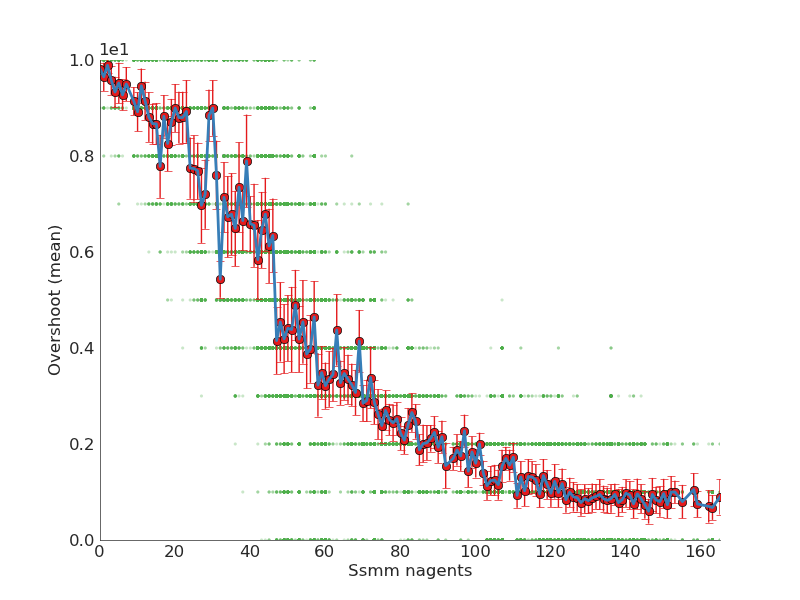
\includegraphics[width=0.5\textwidth]{101_pars_vs_fits/d10/ssmm_nAgents__vs__overshoot(mean)_scatter.png}}
	\subcaptionbox{Correlation between \ssmmnAgents{} and \roundstable\label{fig:d10_parvfit_ssmmnAgents_b}}
	[0.49\linewidth]{\includegraphics[width=0.5\textwidth]{101_pars_vs_fits/d10/ssmm_nAgents__vs__round_stable(mean)_scatter.png}}
	\subcaptionbox{Correlation between \ssmmnAgents{} and \stdev\label{fig:d10_parvfit_ssmmnAgents_c}}
	[0.49\linewidth]{\includegraphics[width=0.5\textwidth]{101_pars_vs_fits/d10/ssmm_nAgents__vs__stdev(mean)_scatter.png}}
	\subcaptionbox{Correlation between \ssmmnAgents{} and \timetoreachnewfundamental\label{fig:d10_parvfit_ssmmnAgents_d}}
	[0.49\linewidth]{\includegraphics[width=0.5\textwidth]{101_pars_vs_fits/d10/ssmm_nAgents__vs__time_to_reach_new_fundamental(mean)_scatter.png}}
	\caption{Correlation between \ssmmnAgents and the four fitness measures in experiment \dten}
	\label{fig:d10_parvfit_ssmmnAgents}
\end{figure}
Figure \ref{fig:d10_parvfit_ssmmnAgents} shows how the number of market makers correlates with the model fitness in experiment \dten. Evidently a large number of market makers reduces the overshoot, whereas the market virtually always have an overshoot when there are few or no market makers. The same is true for the trade prices flicker: few market makers always means flickering prices. A higher number of market makers cause the market to be less responsive, while fewer market makers have the opposite effect. Finally, the number of market makers also influences how quickly the market settles within the stability margin, as markets with more market makers become stable faster than markets with few agents. Table \ref{table:ssmmnagents_quantiles} shows the average fitness values for models where the number of market maker agents was respectively below and above the first ($q_{1}$) and ninth ($q_{9}$) 10-quantiles in the dataset.  The two quantiles were at $q_{1} =46 $ and $q_{9} = 136$. It is seen that the market containing a large number of market makers (more than 136) had a much smaller overshoot, less flickering prices, a slower response time, and stayed within the stability margin faster, compared to the markets with a low (less than 46) number of market makers.

\begin{table}
\centering
\begin{tabular}{lrr}
\toprule
\dten &       $\ssmmnAgents < q_{1}$ &       $\ssmmnAgents > q_{9}$ \\
\midrule
\overshoot                     &     7.5 &     0.8 \\
\roundstable                  & 89876.2 & 18546.9 \\
\stdev              &     1.6 &     0.6 \\
\timetoreachnewfundamental & 12590.5 & 19832.1 \\
\bottomrule
\end{tabular}
\caption{Average fitness values for the market with the top 10\% highest and 10\% lowest number of market makers}
\label{table:ssmmnagents_quantiles}
\end{table}

\subsection{Market maker latency}
The parameters controlling the market maker latency was varied in experiments \dnine, \dten{} and \deleven. However, since the data from \dnine{} turned out to be too noise due to the large number of parameters included in the search, only data from \dten{} and \deleven{} was used. 

\subsubsection*{Fixing the number of chartists}
In experiment \dten, the number of chartists was kept fixed at $\scnAgents = 150$, while \ssmmnAgents was varied by the GA. In this case, the \ssmmlatencymu is found to be somewhat correlated with the fitness measures as illustrated on figure \ref{fig:d10_parvfit_ssmmlatencymu}. Especially for $\ssmmlatencymu > 50$, the data seems to be consistent, as the error bars showing the standard deviation of the data are small in this region. However, for $\ssmmlatencymu < 50$, the model behavior is no longer predictable by using \ssmmlatencymu alone. Figure \ref{fig:faster_mm_makes_worse_markets/d10/MM_mmlatency} shows line plots of the four fitness measures plotted against \ssmmlatencymu. Each line shows the average fitness of markets in which the number of market makers is in a limited range as shown in the legend. The figure shows that even though the market maker latency does influence the market, the effect is secondary to that of the number of agents. For instance, when the market contains less than 25 market makers, all four fitness measures are more or less unchanged, as is evident by the nearly flat red curves. As the number of market makers grow, so does the importance of how fast they are. The average overshoot and the average time to catch up to the new fundamental only change slightly, even with over 100 market makers (yellow line). On the other hand, the average price flickering and the average number of rounds it takes for the market to settle within the stability margin both change significantly with the market maker speed for $\ssmmnAgents > 50$. In summary, figure \ref{fig:faster_mm_makes_worse_markets/d10/MM_mmlatency} shows that in a market with only a few market makers, these agents have little influence no matter how fast they are. As the number of market makers grow, so does the collective force of all the market makers, and so does the importance of how slow or fast these agents are. 
\begin{figure}
	%issue 15
	\centering
	\subcaptionbox{Correlation between \ssmmlatencymu and \overshoot\label{fig:d10_parvfit_ssmmlatencymu_a}}
	[0.49\linewidth]{\includegraphics[width=0.5\textwidth]{101_pars_vs_fits/d10/ssmm_latency_mu__vs__overshoot(mean)_scatter.png}}
	\subcaptionbox{Correlation between \ssmmlatencymu and \roundstable\label{fig:d10_parvfit_ssmmlatencymu_b}}
	[0.49\linewidth]{\includegraphics[width=0.5\textwidth]{101_pars_vs_fits/d10/ssmm_latency_mu__vs__round_stable(mean)_scatter.png}}
	\subcaptionbox{Correlation between \ssmmlatencymu and \stdev\label{fig:d10_parvfit_ssmmlatencymu_c}}
	[0.49\linewidth]{\includegraphics[width=0.5\textwidth]{101_pars_vs_fits/d10/ssmm_latency_mu__vs__stdev(mean)_scatter.png}}
	\subcaptionbox{Correlation between \ssmmlatencymu and \timetoreachnewfundamental\label{fig:d10_parvfit_ssmmlatencymu_d}}
	[0.49\linewidth]{\includegraphics[width=0.5\textwidth]{101_pars_vs_fits/d10/ssmm_latency_mu__vs__time_to_reach_new_fundamental(mean)_scatter.png}}
	\caption{Correlation between \ssmmlatencymu{} and fitness values (fixed \scnAgents, variable \ssmmnAgents)}
	\label{fig:d10_parvfit_ssmmlatencymu}
\end{figure}
Although the influence of $\ssmmlatencymu$ depends on $\ssmmnAgents$, 
. $q_{1}$ and $q_{1}$ 
\begin{table}
\centering
\begin{tabular}{lrr}
\toprule
\dten &       $\ssmmlatencymu < q_{1}$ &       $\ssmmlatencymu > q_{9}$ \\
\midrule
\overshoot                     &     5.6 &     0.9 \\
\roundstable                  & 85927.9 & 18329.3 \\
\stdev                         &     1.4 &     0.6 \\
\timetoreachnewfundamental & 16649.4 & 18795.3 \\
\bottomrule
\end{tabular}
\hspace*{0.4in}
\begin{tabular}{lrr}
\toprule
\deleven &       $\ssmmlatencymu < q_{1}$ &       $\ssmmlatencymu > q_{9}$ \\
\midrule
\overshoot                     &    14.2 &     1.7 \\
\roundstable                  & 81379.2 & 26153.0 \\
\stdev                         &     3.6 &     1.0 \\
\timetoreachnewfundamental & 15856.2 & 18107.4 \\
\bottomrule
\end{tabular}
\caption{Average fitness values for the market with the top 10\% highest and 10\% lowest number of market makers}
\label{table:ssmmlatencymu_quantiles}
\end{table}


The next section will examine how the market behaves with respect to how many chartists are active in the market, and with respect to the latency of the chartists.

\begin{figure}
	%issue 15
	\centering
	\subcaptionbox{\label{fig:faster_mm_makes_worse_markets/d10/overshoot_MM_mmlatency}}
	[0.49\linewidth]{\includegraphics[width=0.5\textwidth]{faster_mm_makes_worse_markets/d10/overshoot_MM_mmlatency.png}}
	\subcaptionbox{\label{fig:faster_mm_makes_worse_markets/d10/round_stable_MM_mmlatency}}
	[0.49\linewidth]{\includegraphics[width=0.5\textwidth]{faster_mm_makes_worse_markets/d10/round_stable_MM_mmlatency.png}}
	\subcaptionbox{\label{fig:faster_mm_makes_worse_markets/d10/stdev_MM_mmlatency}}
	[0.49\linewidth]{\includegraphics[width=0.5\textwidth]{faster_mm_makes_worse_markets/d10/stdev_MM_mmlatency.png}}
	\subcaptionbox{\label{fig:faster_mm_makes_worse_markets/d10/time_to_reach_new_fundamental_MM_mmlatency}}
	[0.49\linewidth]{\includegraphics[width=0.5\textwidth]{faster_mm_makes_worse_markets/d10/time_to_reach_new_fundamental_MM_mmlatency.png}}
	\caption{Relation between \ssmmnAgents, \ssmmlatencymu, and the model fitness when the number of chartists was fixed to $\scnAgents = 150 agents$. Due to missing data, some of the curves are not complete.}
	\label{fig:faster_mm_makes_worse_markets/d10/MM_mmlatency}
\end{figure}




\subsubsection{Fixing the number of market makers}XXXNOT FINISHEDXXX
In experiment \deleven, the number of chartists was varied, while the number of market makers were kept at a constant $\ssmmnAgents = 52$ agents. While it was fairly obvious that the market would not be impacted by changing \ssmmlatencymu when only a few market makers were active, it is less obvious that the same is true for the number of chartists. Yet figure 

\begin{figure}
	%issue 15
	\centering
	\subcaptionbox{Correlation between \ssmmlatencymu and \overshoot\label{fig:d11_parvfit_ssmmlatencymu_a}}
	[0.49\linewidth]{\includegraphics[width=0.5\textwidth]{101_pars_vs_fits/d11/ssmm_latency_mu__vs__overshoot(mean)_scatter.png}}
	\subcaptionbox{Correlation between \ssmmlatencymu and \roundstable\label{fig:d11_parvfit_ssmmlatencymu_b}}
	[0.49\linewidth]{\includegraphics[width=0.5\textwidth]{101_pars_vs_fits/d11/ssmm_latency_mu__vs__round_stable(mean)_scatter.png}}
	\subcaptionbox{Correlation between \ssmmlatencymu and \stdev\label{fig:d11_parvfit_ssmmlatencymu_c}}
	[0.49\linewidth]{\includegraphics[width=0.5\textwidth]{101_pars_vs_fits/d11/ssmm_latency_mu__vs__stdev(mean)_scatter.png}}
	\subcaptionbox{Correlation between \ssmmlatencymu and \timetoreachnewfundamental\label{fig:d11_parvfit_ssmmlatencymu_d}}
	[0.49\linewidth]{\includegraphics[width=0.5\textwidth]{101_pars_vs_fits/d11/ssmm_latency_mu__vs__time_to_reach_new_fundamental(mean)_scatter.png}}
	\caption{Correlation between \ssmmlatencymu{} and fitness values (fixed \ssmmnAgents, variable \scnAgents)}
	\label{fig:d11_parvfit_ssmmlatencymu}
\end{figure}


\begin{figure}
     %issue 15
     \centering
     \subcaptionbox{}
     [0.49\linewidth]{\includegraphics[width=0.5\textwidth]{faster_mm_makes_worse_markets/d11/overshoot_SC_mmlatency.png}}
     \subcaptionbox{}
     [0.49\linewidth]{\includegraphics[width=0.5\textwidth]{faster_mm_makes_worse_markets/d11/round_stable_SC_mmlatency.png}}
     \subcaptionbox{}
     [0.49\linewidth]{\includegraphics[width=0.5\textwidth]{faster_mm_makes_worse_markets/d11/stdev_SC_mmlatency.png}}
     \subcaptionbox{}
     [0.49\linewidth]{\includegraphics[width=0.5\textwidth]{faster_mm_makes_worse_markets/d11/time_to_reach_new_fundamental_SC_mmlatency.png}}
     \caption{Relation between \ssmmnAgents, \ssmmlatencymu, and the model fitness when the number of market makers was fixed to $\ssmmnAgents = 52$ agents.}
     \label{fig:faster_mm_makes_worse_markets/d11/SC_mmlatency}
\end{figure}


\subsection{Number of chartists}
\begin{figure}
	%issue 15
	\centering
	\subcaptionbox{Correlation between \scnAgents and \overshoot\label{fig:d11_parvfit_scnagents_a}}
	[0.49\linewidth]{\includegraphics[width=0.5\textwidth]{101_pars_vs_fits/d11/sc_nAgents__vs__overshoot(mean)_scatter.png}}
	\subcaptionbox{Correlation between \scnAgents and \roundstable\label{fig:d11_parvfit_scnagents_b}}
	[0.49\linewidth]{\includegraphics[width=0.5\textwidth]{101_pars_vs_fits/d11/sc_nAgents__vs__round_stable(mean)_scatter.png}}
	\subcaptionbox{Correlation between \scnAgents and \stdev\label{fig:d11_parvfit_scnagents_c}}
	[0.49\linewidth]{\includegraphics[width=0.5\textwidth]{101_pars_vs_fits/d11/sc_nAgents__vs__stdev(mean)_scatter.png}}
	\subcaptionbox{Correlation between \scnAgents and \timetoreachnewfundamental\label{fig:d11_parvfit_scnagents_d}}
	[0.49\linewidth]{\includegraphics[width=0.5\textwidth]{101_pars_vs_fits/d11/sc_nAgents__vs__time_to_reach_new_fundamental(mean)_scatter.png}}
	\caption{Correlation between \scnAgents and the four fitness measures when $\ssmmnAgents = 52$ (experiment \deleven)}
	\label{fig:d11_parvfit_scnagents}
\end{figure}
Figure \ref{fig:d11_parvfit_scnagents} shows the average population wide number of agents $\E{\scnAgents}$ plotted against each of the four fitness measures, and the figures are summarized below.

\begin{itemize}
\item The more chartists a market has, the faster it responds to the fundamental. This is especially true when comparing markets with less than 100 chartists, and less pronounced when comparing markets with over 100 chartists.
\item The model overshoot is also correlated with the number of chartists in such a way that markets with more chartists have a larger overshoot on average. Whereas the market only seemed to benefit from a decreased response time when the number of chartists were kept below 100, the overshoot continues to grow steadily larger even as the number of chartists is increased beyond 100 agents.
\item \stdev is correlated with the number of chartists in the same way as \overshoot, such that more chartists make the traded prices flicker more.
\item Finally, the graph for \roundstable show that the market rarely becomes stable when it contains more than 50 chartists or so.
\end{itemize}
The large errorbars around the points with a large value of \scnAgents is caused by data sparsity in this region. The GA was set to search for stable markets, and since markets with a large number of chartists tend to be unstable, such markets were rarely selected for creating offspring. 





\subsection{Chartist latency}

\subsubsection*{Fixed number of chartists}

Figure \ref{fig:d10_parvfit_sclatencymu_a} shows that \sclatencymu is negatively correlated with \overshoot, such that markets with faster chartists are more likely to have a larger overshoot.  Next, figure \ref{fig:d10_parvfit_sclatencymu}  shows that \sclatencymu is negatively correlated with \stdev, such that markets with faster chartists are more likely to have flickering trade prices. 

As for the market responsiveness, it is seen that \sclatencymu is positively correlated with \timetoreachnewfundamental, such that markets with faster agents is more likely to have a shorter response time to the market. Figure \ref{fig:d10_parvfit_sclatencymu_d} confirms that markets with fast chartists did actually manage to reach the new fundamental price faster than those markets having slow chartists. The average response time of markets in which the chartists had a latency of less than 30 rounds was around 18000 rounds, whereas it was around 25000 rounds with chartists with more than 100 rounds of latency. The market response time is most sensitive in the range $20< \sclatencymu<60$, and does not change much for larger latencies. 

The plots of \overshoot, \stdev and \timetoreachnewfundamental show that predicting the three fitness measures in markets with slow chartists would be more accurate than for markets with fast chartists, as the correlation of \overshoot, \stdev and \timetoreachnewfundamental with \sclatencymu is stronger for larger values of \sclatencymu. 

Figure \ref{fig:d10_parvfit_sclatencymu_b} shows that \sclatencymu is positively correlated with \roundstable, but also that the relationship between \sclatencymu and \roundstable seems highly non-linear. The figure illustrates the binary nature of the stability criteria, that is, that a simulation is either stable or not stable. This causes \roundstable to have a high conditional variance of \roundstable given \sclatencymu in the region $50 < \sclatencymu < 120$, meaning that that prediction of \roundstable from \sclatencymu in this region would not be very accurate. What this means is that the stability of a simulation is highly dependent on factors other than \sclatencymu, when the parameter is within 50 to 120 rounds. When the chartists are faster than 50 rounds, the market is almost always unstable, and when the chartists are slower than 120 rounds the market is almost always stable. 

\begin{figure}
	%issue 15
	\centering
	\subcaptionbox{Correlation between \sclatencymu and \overshoot\label{fig:d10_parvfit_sclatencymu_a}}
	[0.49\linewidth]{\includegraphics[width=0.5\textwidth]{101_pars_vs_fits/d10/sc_latency_mu__vs__overshoot(mean)_scatter.png}}
	\subcaptionbox{Correlation between \sclatencymu and \roundstable\label{fig:d10_parvfit_sclatencymu_b}}
	[0.49\linewidth]{\includegraphics[width=0.5\textwidth]{101_pars_vs_fits/d10/sc_latency_mu__vs__round_stable(mean)_scatter.png}}
	\subcaptionbox{Correlation between \sclatencymu and \stdev\label{fig:d10_parvfit_sclatencymu_c}}
	[0.49\linewidth]{\includegraphics[width=0.5\textwidth]{101_pars_vs_fits/d10/sc_latency_mu__vs__stdev(mean)_scatter.png}}
	\subcaptionbox{Correlation between \sclatencymu and \timetoreachnewfundamental\label{fig:d10_parvfit_sclatencymu_d}}
	[0.49\linewidth]{\includegraphics[width=0.5\textwidth]{101_pars_vs_fits/d10/sc_latency_mu__vs__time_to_reach_new_fundamental(mean)_scatter.png}}
	\caption{Correlation between chartist latency and fitness values (fixed \scnAgents, variable \ssmmnAgents)}
	\label{fig:d10_parvfit_sclatencymu}
\end{figure}

\begin{figure}
	%issue 15
	\centering
	\subcaptionbox{\label{fig:faster_mm_makes_worse_markets/d10/overshoot_MM_sclatency}}
	[0.49\linewidth]{\includegraphics[width=0.5\textwidth]{faster_mm_makes_worse_markets/d10/overshoot_MM_sclatency.png}}
	\subcaptionbox{\label{fig:faster_mm_makes_worse_markets/d10/round_stable_MM_sclatency}}
	[0.49\linewidth]{\includegraphics[width=0.5\textwidth]{faster_mm_makes_worse_markets/d10/round_stable_MM_sclatency.png}}
	\subcaptionbox{\label{fig:faster_mm_makes_worse_markets/d10/stdev_MM_sclatency}}
	[0.49\linewidth]{\includegraphics[width=0.5\textwidth]{faster_mm_makes_worse_markets/d10/stdev_MM_sclatency.png}}
	\subcaptionbox{\label{fig:faster_mm_makes_worse_markets/d10/time_to_reach_new_fundamental_MM_sclatency}}
	[0.49\linewidth]{\includegraphics[width=0.5\textwidth]{faster_mm_makes_worse_markets/d10/time_to_reach_new_fundamental_MM_sclatency.png}}
	\caption{Relation between \ssmmnAgents, \sclatencymu, and the model fitness when the number of chartists was fixed to $\scnAgents = 150 agents$. Due to missing data, some of the curves are not complete.}
	\label{fig:faster_mm_makes_worse_markets/d10/MM_sclatency}
\end{figure}




\subsubsection*{Fixed number of market makers}

\begin{figure}
	%issue 15
	\centering
	\subcaptionbox{Correlation between \sclatencymu and \overshoot\label{fig:d11_parvfit_sclatencymu_a}}
	[0.49\linewidth]{\includegraphics[width=0.5\textwidth]{101_pars_vs_fits/d11/sc_latency_mu__vs__overshoot(mean)_scatter.png}}
	\subcaptionbox{Correlation between \sclatencymu and \roundstable\label{fig:d11_parvfit_sclatencymu_b}}
	[0.49\linewidth]{\includegraphics[width=0.5\textwidth]{101_pars_vs_fits/d11/sc_latency_mu__vs__round_stable(mean)_scatter.png}}
	\subcaptionbox{Correlation between \sclatencymu and \stdev\label{fig:d11_parvfit_sclatencymu_c}}
	[0.49\linewidth]{\includegraphics[width=0.5\textwidth]{101_pars_vs_fits/d11/sc_latency_mu__vs__stdev(mean)_scatter.png}}
	\subcaptionbox{Correlation between \sclatencymu and \timetoreachnewfundamental\label{fig:d11_parvfit_sclatencymu_d}}
	[0.49\linewidth]{\includegraphics[width=0.5\textwidth]{101_pars_vs_fits/d11/sc_latency_mu__vs__time_to_reach_new_fundamental(mean)_scatter.png}}
	\caption{Correlation between chartist latency and fitness values (fixed \ssmmnAgents, variable \scnAgents)}
	\label{fig:d11_parvfit_sclatencymu}
\end{figure}

\begin{figure}
     %issue 15
     \centering
     \subcaptionbox{}
     [0.49\linewidth]{\includegraphics[width=0.5\textwidth]{faster_mm_makes_worse_markets/d11/overshoot_SC_sclatency.png}}
     \subcaptionbox{}
     [0.49\linewidth]{\includegraphics[width=0.5\textwidth]{faster_mm_makes_worse_markets/d11/round_stable_SC_sclatency.png}}
     \subcaptionbox{}
     [0.49\linewidth]{\includegraphics[width=0.5\textwidth]{faster_mm_makes_worse_markets/d11/stdev_SC_sclatency.png}}
     \subcaptionbox{}
     [0.49\linewidth]{\includegraphics[width=0.5\textwidth]{faster_mm_makes_worse_markets/d11/time_to_reach_new_fundamental_SC_sclatency.png}}
     \caption{Relation between \scnAgents, \sclatencymu, and the model fitness when the number of market makers was fixed to $\ssmmnAgents = 52$ agents.}
     \label{fig:faster_mm_makes_worse_markets/d11/SC_sclatency}
\end{figure}

Figures \ref{fig:d11_parvfit_sclatencymu} seems to indicate that no correlations exist between the speed of the chartist agents, and the model fitness measures. However, since figure \ref{fig:d10_parvfit_sclatencymu} does point towards the existence of such correlations, something else must be obscuring the scatter plots in \ref{fig:d11_parvfit_sclatencymu}. The reason is found to be that the number of chartists was not kept constant in experiment \deleven. It turns out that \sclatencymu{} is in fact correlated with \overshoot, \stdev and \timetoreachnewfundamental, but that the correlation depends heavily on the number of chartists in the market. 






\subsection{Chartist to market maker ratio}
\begin{figure}
	%issue 15
	\centering
	\subcaptionbox{}
	[0.49\linewidth]{\includegraphics[width=0.5\textwidth]{101_pars_vs_fits/d10/chartist_per_market_maker__vs__overshoot(mean)_scatter.png}}
	\subcaptionbox{}
	[0.49\linewidth]{\includegraphics[width=0.5\textwidth]{101_pars_vs_fits/d10/chartist_per_market_maker__vs__round_stable(mean)_scatter.png}}
	\subcaptionbox{}
	[0.49\linewidth]{\includegraphics[width=0.5\textwidth]{101_pars_vs_fits/d10/chartist_per_market_maker__vs__stdev(mean)_scatter.png}}
	\subcaptionbox{}
	[0.49\linewidth]{\includegraphics[width=0.5\textwidth]{101_pars_vs_fits/d10/chartist_per_market_maker__vs__time_to_reach_new_fundamental(mean)_scatter.png}}
	\caption{Correlations between \ratioagents and the fitness values when $\scnAgents = 150$}
	\label{fig:parvfit_ratio_d10}
\end{figure}
The above observations about how the number of agents influence the stability and speed of the market pointed out that more market makers made the market slow but stable, while more chartists made the market fast, but unstable. By merging \datamatrixpar{\dten} and \datamatrixpar{\deleven}, we can calculate the ratio, \ratioagents, between the number of chartists and the number of market makers, and see how the fitness values correlate. Figure \ref{fig:parvfit_ratio} shows the resulting scatter plots. 

\begin{figure}
	%issue 15
	\centering
	\subcaptionbox{}
	[0.49\linewidth]{\includegraphics[width=0.5\textwidth]{101_pars_vs_fits/d11/chartist_per_market_maker__vs__overshoot(mean)_scatter.png}}
	\subcaptionbox{}
	[0.49\linewidth]{\includegraphics[width=0.5\textwidth]{101_pars_vs_fits/d11/chartist_per_market_maker__vs__round_stable(mean)_scatter.png}}
	\subcaptionbox{}
	[0.49\linewidth]{\includegraphics[width=0.5\textwidth]{101_pars_vs_fits/d11/chartist_per_market_maker__vs__stdev(mean)_scatter.png}}
	\subcaptionbox{}
	[0.49\linewidth]{\includegraphics[width=0.5\textwidth]{101_pars_vs_fits/d11/chartist_per_market_maker__vs__time_to_reach_new_fundamental(mean)_scatter.png}}
	\caption{Correlations between \ratioagents and the fitness values when $\ssmmnAgents = 52$}
	\label{fig:parvfit_ratio_d11}
\end{figure}








\section{Grouping models by behavior}
This section is be concerned with trying to tie various patterns of model behavior to different regions in the parameter space. The quickest way to get an idea of how the data generated by the simulations is distributed is to make scatter plots. Scatter plots are probably among the most rudimentary of techniques for data analysis, yet they can be incredibly informative, especially when the data that is visualized is low-dimensional. The data of the model fitness is four-dimensional, requiring twelve plots to visualize all combinations. However, since \overshoot is discrete with a small range of values, it is not suitable for a scatter plot. Furthermore, some scatter plots are not useful for interpretation if they do not show any structure in the data. Figure \ref{figure:d9_scatter_fitness} shows three scatter plots which were found to best illustrate the structure of the dataset from \dnine. Note also that coloring each point corresponding to its value in one dimension makes it possible to show how the data is distributed in three dimensions.
\begin{figure}
\centering
\subcaptionbox{$\log \stdev$ vs. $\log \roundstable$ vs. \timetoreachnewfundamental}
[0.49\linewidth]{\includegraphics[width=0.5\textwidth]{21_scatter_plots/d9/d.png}}
\subcaptionbox{\roundstable vs. \timetoreachnewfundamental vs. \stdev}
[0.49\linewidth]{\includegraphics[width=0.5\textwidth]{21_scatter_plots/d9/c.png}}
\subcaptionbox{$\log \overshoot$ vs . $\log \stdev$ vs. \timetoreachnewfundamental}
[0.49\linewidth]{\includegraphics[width=0.5\textwidth]{21_scatter_plots/d9/b.png}}
\caption{Scatter plots of fitness measures in experiment \dnine. }
\label{figure:d9_scatter_fitness}
\end{figure}
The scatter plots do seem to reveal some structure, the presence of large values in the \stdev feature obscures the nature of this structure, in spite of the logarithmic scaling. The plot showing $\log \stdev$ vs. $\log \roundstable$ is squeezed to the left, and the color grading on the scatter plot for $\log \overshoot$ vs . $\log \stdev$ reveals no variety in the \stdev feature. In an attempt to get some more information out of the scatter plot, data points with an overshoot of over 100 \% of the shock to the fundamental (corresponding to $\overshoot > 10$ ) are removed. The resulting scatter plots for the reduced data set are shown on figures \ref{figure:scatter_fitness_inliers_a} and \ref{figure:scatter_fitness_inliers_b}.

First of all, it is seen that while the data is distributed similarly in the three data sets, there are some differences. The data from \dnine{} seems to have many ``lonely'' data points, which are not part of any cluster, whereas the data from \dten{} somehow seems to be the cleanest of the three. In all three data sets, there are clusters of data. The clusters do not necessarily mean anything in themselves. They might simply be due to the way that data points are mutated and crossed by the GA. However, by considering which regions of the fitness space that each cluster covers, it is possible to add meaning to the clusters in terms of model behavior.

\begin{figure}
\centering
\subcaptionbox{Experiment \dnine}[0.49\linewidth]{\includegraphics[width=0.5\textwidth]{103_scatter_manual_outlier/d9/f.png}}
\subcaptionbox{Experiment \dnine}[0.49\linewidth]{\includegraphics[width=0.5\textwidth]{103_scatter_manual_outlier/d9/j.png}}
\subcaptionbox{Experiment \dten}[0.49\linewidth]{\includegraphics[width=0.5\textwidth]{103_scatter_manual_outlier/d10/f.png}}
\subcaptionbox{Experiment \dten}[0.49\linewidth]{\includegraphics[width=0.5\textwidth]{103_scatter_manual_outlier/d10/j.png}}
\subcaptionbox{Experiment \deleven}[0.49\linewidth]{\includegraphics[width=0.5\textwidth]{103_scatter_manual_outlier/d11/f.png}}
\subcaptionbox{Experiment \deleven}[0.49\linewidth]{\includegraphics[width=0.5\textwidth]{103_scatter_manual_outlier/d11/j.png}}
\caption{Scatter plot of \roundstable against \timetoreachnewfundamental with coloring showing $\log \stdev$ and \overshoot}
\label{figure:scatter_fitness_inliers_a}
\end{figure}

\begin{figure}
\centering
\subcaptionbox{Experiment \dnine}[0.49\linewidth]{\includegraphics[width=0.5\textwidth]{103_scatter_manual_outlier/d9/h.png}}
\subcaptionbox{Experiment \dnine}[0.49\linewidth]{\includegraphics[width=0.5\textwidth]{103_scatter_manual_outlier/d9/k.png}}
\subcaptionbox{Experiment \dten}[0.49\linewidth]{\includegraphics[width=0.5\textwidth]{103_scatter_manual_outlier/d10/h.png}}
\subcaptionbox{Experiment \dten}[0.49\linewidth]{\includegraphics[width=0.5\textwidth]{103_scatter_manual_outlier/d10/k.png}}
\subcaptionbox{Experiment \deleven}[0.49\linewidth]{\includegraphics[width=0.5\textwidth]{103_scatter_manual_outlier/d11/h.png}}
\subcaptionbox{Experiment \deleven}[0.49\linewidth]{\includegraphics[width=0.5\textwidth]{103_scatter_manual_outlier/d11/k.png}}
\caption{Scatter plot of $\log \stdev$ against \timetoreachnewfundamental with coloring showing $\roundstable$ and \overshoot}
\label{figure:d9_scatter_fitness_inliers_b}
\end{figure}



\subsection{Manually grouping simulations by behavior}\label{section:manually_grouping_simulations}
Table \ref{table:manual_filtering} contains an overview of the named criteria used for roughly grouping simulations into different types of behavior. The following text contains the reasoning for why each of these groups are interesting.

In figure \ref{figure:scatter_fitness_inliers_a}, the black dashed lines at $\timetoreachnewfundamental = \roundstable$ divide each plot into region A, (upper left triangle) and region B (lower right triangle). Region A contains the fitness-points of the simulations which are counted as stable \textit{after} they reach the new fundamental, and region B contain those that become stable before. 

The description below provides a brief summary of which simulations belong in the two regions.
\begin{description}
\item[$\roundstable < \timetoreachnewfundamental$] This happens when the traded price never leaves the stability margin after reaching the new fundamental price. Note however that this case does not necessarily mean that the prices do not flicker. 
\item[$\roundstable > \timetoreachnewfundamental$] This happens when the traded price leaves the stability margin once or more after reaching the new fundamental. The traded price can be close to the fundamental, but flickers in and out of the stability margin as on Figure \ref{figure:tradeprice_exaples_fitness_a} shows an example where the trade price fairly stable and with no overshoot, leading to good (low) \stdev and \overshoot fitness values to be assigned to the parameters. However, even though the traded prices are mostly within the stability margin, occasional flickers out of the margin causes the simulation to score a bad (high) \roundstable fitness. Note also that \timetoreachnewfundamental is undefined in this case. 
\item[$\roundstable = \timetoreachnewfundamental$] This happens if a trade is executed at price $\smargin - \fas < \pmatch < \smargin + \fas$, and another trade is executed at price $\pmatch = \fas$ in the same round. 
\end{description}


\subsubsection*{Fast and stable simulations with flickering prices}
The points in the lower left corner in are those which quickly reached the new fundamental price, and quickly because stable, leading those simulations to be assigned low \timetoreachnewfundamental and \roundstable fitness-values. These points are extracted by using filter F1 (see table \ref{table:manual_filtering})

\subsubsection*{Slow or fast and stable simulations with non-flickering prices}
All three data sets have data points which are close to the diagonal. However, only \dnine{} has data points which are close to the diagonal in the upper right corner of the figure. These points are interesting because they belong to simulations which became stable as soon as they reached the new fundamental price. Hence, these simulations should have prices that do not flicker, and therefore yield a small \stdev-fitness. This is confirmed by looking at the left scatter plot of \dnine, as all the points close to the dotted line has a green/blue color. The right plot of \dnine{} shows that these simulations did not have any overshoot. It is interesting that both slow simulations which take a long time to reach the new fundamental, as well as simulations who manage to be fast, have no overshoot, and this observation begs the question of whether or not these simulations have some common parameters that make them behave in such a way. These points are extracted by applying filters F2 and F3 (see table \ref{table:manual_filtering}) to the data matrix \datamatrixfit{\dnine} which selects points that lie within a distance of 400 rounds of the diagonal. 


\subsubsection*{Stable before reaching the new fundamental}
Most of the simulations falling in region B, meaning that they became stable before reaching the new fundamental price, had no overshoot. However, when the model was allowed to have a large number of chartists, but in \deleven, a group of simulations did have a small overshoot. These two groups of points were extracted by applying filters F4 and F5  (see table \ref{table:manual_filtering}).

\subsubsection*{Simulations with overshoot}
XXX NOT FINISHED

\subsubsection{Fast simulations}
All three experiments produces a group of simulations which had a quick response to the shock, but took longer to become stable. The simulations are in the column-shaped cluster in figure \ref{figure:scatter_fitness_inliers_a} and the all have relatively low \timetoreachnewfundamental-fitness of less than 25000 rounds or so. These data points were extracted using filters F7 and F8 (see table \ref{table:manual_filtering}).

\subsubsection*{Unstable simulations with non-flickering prices}
The final group of simulation that are singles out in this section are those that had very smooth price curves (that is, a small value for \stdev), yet did not manage to become stable. These simulations were selected by filter F9.

\begin{figure}
\centering
\subcaptionbox{Experiment \dnine}[0.32\linewidth]{\includegraphics[width=0.32\textwidth]{manual_filtering/d9/group_overlap.png}\label{figure:jaccard_index_a}}
\subcaptionbox{Experiment \dnine}[0.32\linewidth]{\includegraphics[width=0.32\textwidth]{manual_filtering/d10/group_overlap.png}\label{figure:jaccard_index_b}}
\subcaptionbox{Experiment \dten}[0.32\linewidth]{\includegraphics[width=0.32\textwidth]{manual_filtering/d11/group_overlap.png}\label{figure:jaccard_index_c}}
\caption{Jaccard index between the sets of data points extracted by each filter}
\label{figure:jaccard_index}
\end{figure}

The criteria in table \ref{table:manual_filtering} do not prevent a simulation to be selected by different filters. The groups of points are therefore likely to have a non-empty intersection. Using the filters is an the attempt to separate the simulations by their behavior. Hence, the filters should in general not select the same data points. The Jaccard index $J(A,B)$ is calculated between sets $A$ and $B$ and used to determine the overlap between the sets. Figure \ref{figure:jaccard_index} shows the Jaccard index between the sets created by applying the filters to each of the three data sets. Since the distance matrix is symmetrical, only the upper left part has been plotted. In case that the filter produced an empty set, the Jaccard index is undefined, resulting in white squares.

\begin{equation}
J(A,B) = \frac{\lvert A \cap B \rvert}{\lvert A \cup B\rvert }
\end{equation}

\begin{equation}
J(A,B) = \frac{\lvert A \cap B \rvert}{\min \lvert A \rvert, \lvert B\rvert }
\end{equation}


\begin{table}
\centering
\begin{tabular}{l|E|l|E}
\toprule
ID & Target simulations & Filter criteria\\
\midrule
F1 & Fast and stable (but maybe flickering) & $\timetoreachnewfundamental < 12000$, $\roundstable < 12000$, $\log \stdev > 0$ \\
\midrule
F2 & Slow, stable and not flickering (diagonal)& $\lvert \timetoreachnewfundamental - \roundstable \rvert < 400$\\
\midrule 
F3 & Fast and stable and not flickering (diagonal)& $\lvert \timetoreachnewfundamental - \roundstable \rvert < 400$\\
\midrule
F4 & Stable before reaching fundamental, no overshoot& $\roundstable < \timetoreachnewfundamental$, $\overshoot = 0$\\
\midrule
F5 & Stable before reaching fundamental, with overshoot& $\roundstable < \timetoreachnewfundamental$, $\overshoot = >$\\
\midrule
F6 & Has overshoot & $\roundstable > \timetoreachnewfundamental$, $\overshoot > 0$ \\
\midrule
F7 & Fast response, quick to stabilize & $1000 < \timetoreachnewfundamental < 25000$, $20000 < \roundstable < 40000$ \\
\midrule
F8 & Fast response, slow to stabilize & $1000 < \timetoreachnewfundamental < 25000$, $40000 < \roundstable < 75000$ \\
\midrule
F9 & Smooth prices with a small overshoot, yet unstable & $e^{-0.5} - 0.1 < \log \stdev < e^{-0.5} + 0.1$ \\
\midrule
\bottomrule
\end{tabular}
\caption{Filter IDs and fitness-regions}
\label{table:manual_filtering}
\end{table}

\begin{table}
 \centering
 \begin{tabular}{l|rrrrrrrrr}
\toprule
{} &      F1 &      F2 &      F3 &      F4 &      F5 &      F6 &      F7 &      F8 &      F9 \\
\midrule
\sclatencymu                 &    70.1 &    65.5 &    49.5 &    81.5 &    76.7 &    58.5 &    75.8 &    75.6 &    76.0 \\
 \sclatencys                 &     5.4 &     5.5 &     7.8 &     4.5 &     4.9 &     6.8 &     5.0 &     4.9 &     5.0 \\
 \scthinkmu                  &    59.7 &    58.8 &    51.8 &    70.1 &    65.8 &    53.5 &    65.7 &    64.8 &    65.9 \\
 \scthinks                   &    12.0 &    12.0 &    12.8 &    11.2 &    11.6 &    11.2 &    11.4 &    11.6 &    11.6 \\
 \sctimehorizonmu            &  1744.0 &  1676.1 &  1758.1 &  1766.8 &  1773.6 &  1906.9 &  1795.3 &  1757.2 &  1777.9 \\
 \sctimehorizons             &  1483.2 &  1472.7 &  1573.4 &  1415.7 &  1444.2 &  1346.7 &  1437.3 &  1442.4 &  1465.4 \\
 \scwaitTimeBetweenTradingmu &    29.5 &    27.4 &    29.3 &    30.5 &    30.0 &    28.6 &    30.0 &    29.7 &    29.9 \\
 \scwaitTimeBetweenTradings  &     3.2 &     4.1 &     4.2 &     3.0 &     3.1 &     5.1 &     3.1 &     3.0 &     3.1 \\
 \ssmmlatencymu              &    45.2 &    38.5 &    37.6 &    49.8 &    47.3 &    39.2 &    46.1 &    46.3 &    44.5 \\
 \ssmmlatencys               &     4.2 &     4.9 &     4.6 &     4.3 &     4.4 &     5.4 &     4.1 &     4.2 &     5.1 \\
 \ssmmthinkmu                &    39.8 &    38.2 &    40.1 &    37.9 &    38.6 &    35.5 &    39.0 &    39.1 &    35.5 \\
 \ssmmthinks                 &     0.0 &     0.0 &     0.0 &     0.0 &     0.0 &     3.6 &     0.0 &     0.3 &     0.2 \\
 \midrule
\overshoot                   &     1.0 &     1.1 &     1.3 &     0.0 &     1.0 &     3.9 &     1.9 &     2.1 &     1.4 \\
 \roundstable                & 11712.3 & 44993.4 & 13454.5 & 13121.9 & 13468.1 & 80410.6 & 26840.4 & 61259.6 & 54143.9 \\
 \stdev                      &     1.2 &     0.7 &     0.7 &     0.6 &     0.7 &     1.1 &     0.8 &     0.9 &     0.6 \\
 \timetoreachnewfundamental  & 13767.0 & 45089.4 & 13579.4 & 15564.3 & 16743.6 & 16513.3 & 17502.8 & 16812.7 & 40564.2 \\
 \midrule
Count                        &   498 &    33 &  1031 & 33928 & 41982 & 30468 &  2016 &  1733 &  2160 \\
\bottomrule
\end{tabular}
 \label{table:manual_filtering_d9}
 \caption{XXX}
 \end{table}
\begin{table}
 \centering
 \begin{tabular}{l|rrrrrrrrr}
\toprule
{} &      F1 &  F2 &  F3 &      F4 &      F5 &      F6 &      F7 &      F8 &      F9 \\
\midrule
\sclatencymu                &   N/A & N/A & N/A &   123.8 &   121.5 &    78.3 &   116.9 &   104.2 &    95.0 \\
 \sclatencys                &    N/A & N/A & N/A &     6.5 &     6.5 &     9.0 &     7.1 &     8.7 &     8.7 \\
 \ssmmlatencymu             &    N/A & N/A & N/A &    73.9 &    75.8 &    39.2 &    73.3 &    59.6 &    35.9 \\
 \ssmmlatencys              &     N/A & N/A & N/A &     5.6 &     6.0 &     9.6 &     6.6 &     8.7 &     9.2 \\
 \ssmmnAgents               &   N/A & N/A & N/A &   126.5 &   125.6 &    67.1 &   121.2 &    98.0 &    81.2 \\
 \midrule
\overshoot                  &     N/A & N/A & N/A &     0.0 &     1.0 &     4.1 &     1.8 &     2.1 &     0.2 \\
 \roundstable               & N/A & N/A & N/A & 17025.9 & 15920.1 & 81539.2 & 27387.5 & 59444.5 & 24392.3 \\
 \stdev                     &     N/A & N/A & N/A &     0.6 &     0.7 &     1.2 &     0.7 &     0.9 &     0.6 \\
 \timetoreachnewfundamental & N/A & N/A & N/A & 20405.2 & 18724.9 & 15504.3 & 18725.1 & 16840.5 & 31017.6 \\
 \midrule
Count                       &     0 & 0 & 0 &  8486 & 25574 & 47493 &  5379 &  2528 &   399 \\
\bottomrule
\end{tabular}
 \label{table:manual_filtering_d10}
 \caption{XXX}
 \end{table}
\begin{table}
 \centering
 \begin{tabular}{l|rrrrrrrrr}
\toprule
{} &      F1 &  F2 &  F3 &      F4 &      F5 &      F6 &      F7 &      F8 &      F9 \\
\midrule
\sclatencymu                &    N/A & N/A & N/A &    30.4 &    32.3 &    33.3 &    34.3 &    35.1 &    35.8 \\
 \sclatencys                &     N/A & N/A & N/A &     9.3 &     9.9 &     4.6 &     7.2 &     6.6 &     9.0 \\
 \scnAgents                 &    N/A & N/A & N/A &    19.0 &    26.9 &   154.0 &    46.3 &    54.6 &    41.1 \\
 \ssmmlatencymu             &    N/A & N/A & N/A &    67.2 &    55.0 &    38.9 &    50.0 &    47.3 &    46.0 \\
 \ssmmlatencys              &    N/A & N/A & N/A &     8.4 &    11.6 &    22.9 &    17.5 &    19.5 &    14.7 \\
\midrule
\overshoot                  &     N/A & N/A & N/A &     0.0 &     1.0 &    14.6 &     2.0 &     2.6 &     0.0 \\
 \roundstable               & N/A & N/A & N/A & 15678.2 & 15075.3 & 87971.4 & 31954.9 & 63613.9 & 21851.4 \\
 \stdev                     &     N/A & N/A & N/A &     0.7 &     0.8 &     3.6 &     0.9 &     1.0 &     0.6 \\
 \timetoreachnewfundamental & N/A & N/A & N/A & 19965.3 & 18765.4 & 13685.0 & 17265.5 & 16449.5 & 31048.9 \\
 \midrule
Count                       &     0 & 0 & 0 & 71329 & 31377 & 84597 &   349 &  3014 &  1706 \\
\bottomrule
\end{tabular}
 \label{table:manual_filtering_d11}
 \caption{XXX}
 \end{table}
 
Tables \ref{table:manual_filtering_d9}, \ref{table:manual_filtering_d10} and \ref{table:manual_filtering_d11} show the fitness and parameter arithmetic means for each of the nine groups selected by the filters
 
When the number of chartists were fixed as in experiment \dten, the simulations with overshoot (picked out by filter F6) has an average overshot of $\Efilter{6}{\overshoot} = 4.1$ ticks. These markets had comparatively few, but fast market makers ($\Efilter{6}{\ssmmnAgents} = 67.1$ and $\Efilter{6}{\ssmmlatencymu}$), and fast chartists ($\Efilter{6}{\sclatencymu} = 78.3$). Figure \ref{figure:jaccard_index_b} shows that F7 and F8 mostly contain points that are also contained in F6. Both F7 and F8 a lower average overshoot, and this is caused by the markets to have slower chartists, and fewer, slower market makers. When the number of chartists were varied as in experiment \deleven{} (and with a constant of $\ssmmnAgents=52$ market makers), the average latency of the chartists $\Efilter{6}{\sclatencymu}$ did not differ from the other groups. Instead, the biggest difference was that markets with overshoot on average had a high number of chartists. As for the market maker latency, it was smaller than any of the other groups. On the the other hand, markets with no overshoot on average had a large number of marker makers when \scnAgents is fixed to $\scnAgents = 150$, although the market makers were not particularly fast. Markets with no overshoot also had the lowest average number of chartists among the nine groups.

\subsection{Using clustering algorithms to group markets by behavior}\label{section:clustering}

\subsection{Clustering with mixture of Gaussians}
In this section, the focus is shifted from looking at population wide statistics to analysis sub-groups within each population. Whereas the previous sections showed that there do indeed exist statistical relationships between the latency of the agents and the behavior of the model, each discovered correlation was calculated over the entire population. Although the correlations reveal overall tendencies of the model behavior when changing a single parameter, little can be said about how the various parameters interact to determine model behavior. For instance, even though prediction of, say a negative correlation between \timetoreachnewfundamental was \sclatencymu was found, there might be configurations of the model in which faster chartists were actually beneficial to the market. 

One way to approach this problem is to see whether or not there exists relationships between partitions in the parameter space to partitions in the fitness space. As in section \ref{section:filtering_parameters}, the first step is to partition space, since each partition can be interpreted in terms of the model behavior. For instance, a partition covering the lower left half of the 2-dimensional space in figure \ref{figure:scatter_fitness_inliers_a} would encompass all the simulations which had a fast response time and became stable quickly (no matter if they had prices that flickered within the stability margin or not).

In order to investigate this, a Gaussian mixture model (GMM) was used to find clusters in the fitness space. All four fitness measures were used for the clustering. After discarding simulations with undefined fitness values and removing outliers, the data set contained 80813 data points. The large number of data points and the low number of dimensions made it possible to allow a each Gaussian component to have a full covariance matrix, giving the model a high level of flexibility. Figure \ref{fig:d10_scatter_clusters} shows scatter plots of the data after it has been grouped. Tables \ref{table:fit_gmm_all_mean} and \ref{table:fit_gmm_all_std} respectively show the mean and standard deviation calculated over each cluster. The tables are sorted by the average value of \overshoot.



\begin{figure}
	%issue 15
	\centering
	\subcaptionbox{}[0.49\linewidth]{\includegraphics[width=0.5\textwidth]{manually_selected/108_cluster_after_removing_outliers/d10/12_gmm_all_fit_0.png}}
	\subcaptionbox{}[0.49\linewidth]{\includegraphics[width=0.5\textwidth]{manually_selected/108_cluster_after_removing_outliers/d10/12_gmm_all_fit_1.png}}
	\subcaptionbox{}[0.49\linewidth]{\includegraphics[width=0.5\textwidth]{manually_selected/108_cluster_after_removing_outliers/d10/12_gmm_all_fit_2.png}}
	\caption{Scatter plots in fitness space showing the grouping of data points when using a GMM with 12 clusters.}
	\label{fig:d10_scatter_clusters}
\end{figure}

XXX NOT FINISHED. WRITE ABOUT THE CLUSTERS THAT HAVE SOME INTERPRETABLE VALUE. IT DOES NOT HAVE TO BE ALL OF THEM.
$\Varcluster{\roundstable}{8}$ and $\Varcluster{\roundstable}{11}$ and $\Varcluster{\roundstable}{5}$ are large. The points in this cluster have parameters which 



\subsubsection*{Chartist latency and market response time}
As was noted earlier, the evolution of \sclatencymu and \timetoreachnewfundamental indicates that slow chartists made the market slow, and fast chartists made the market fast. C1 is the cluster with the $\Ecluster{\timetoreachnewfundamental}{1}$

\begin{table}
 \centering
 \begin{tabular}{l|rrrr|rrrrr|r}
\toprule
{} &  \overshoot &  \roundstable &  \stdev &  \timetoreachnewfundamental &  \sclatencymu &  \sclatencys &  \ssmmlatencymu &  \ssmmlatencys &  \ssmmnAgents &  \Count \\
\midrule
C1  &         0.0 &       16301.2 &     0.6 &                     19217.4 &         127.2 &          6.2 &            78.4 &            5.2 &         132.2 &  7803 \\
C7  &         0.3 &       24383.1 &     0.7 &                     32005.5 &          87.0 &          9.5 &            25.8 &           10.5 &          66.7 &  1012 \\
C10 &         1.0 &       15832.8 &     0.7 &                     18602.8 &         121.9 &          6.5 &            76.3 &            6.0 &         126.3 & 25245 \\
C8  &         2.0 &       81599.7 &     0.9 &                     16333.6 &         101.8 &          8.7 &            56.4 &            9.2 &          91.3 &  7442 \\
C11 &         2.0 &       30515.0 &     0.7 &                     17822.9 &         114.2 &          7.3 &            71.7 &            7.0 &         117.5 &  5056 \\
C0  &         3.0 &       89015.0 &     1.1 &                     14687.5 &          89.0 &          9.2 &            39.5 &           10.0 &          66.8 &  9201 \\
C5  &         3.0 &       51306.4 &     0.9 &                     16508.7 &         102.2 &          9.0 &            59.2 &            8.8 &          96.0 &   356 \\
C6  &         3.0 &       83914.2 &     1.1 &                     16820.9 &          92.3 &          9.2 &            40.6 &           10.0 &          72.4 &  1598 \\
C9  &         4.0 &       89496.0 &     1.2 &                     14459.8 &          77.7 &          9.6 &            29.9 &           10.4 &          56.7 &  7278 \\
C4  &         5.0 &       89896.6 &     1.4 &                     22034.2 &          62.4 &          9.4 &            21.5 &           10.3 &          51.6 &  5331 \\
C3  &         6.7 &       86440.9 &     1.8 &                     18692.7 &          54.9 &          9.2 &            26.2 &           10.5 &          38.0 &   390 \\
C2  &         7.9 &       89996.1 &     1.6 &                     11574.7 &          36.4 &          9.2 &            26.4 &            9.6 &          36.4 &  10101 \\
Outliers  &        11.5 &       89998.8 &     2.2 &                      8835.1 &          17.8 &          9.3 &            24.3 &            8.5 &          19.4 &   740 \\
\bottomrule
\end{tabular}
 \label{table:d10_gmm_mean}
 \caption{Cluster means (\dten)}
 \end{table}
 
 
 \begin{comment}
 C2 contains the fastest simulations, which take an average of $11.5\times 10^3$ rounds to reach the new fundamental. This group is also the one with the largest overshoot. 
 
 
C7 contains simulations 


Mareket makers are the agents that respond to 


Slow trader match chartist coeincidence
Instead mm match chartists 
If 
Due to the high latency of the slow traders, any order submitted by a slow trader matchng a chartist order i

 \end{comment}

\begin{comment}
\begin{table}
 \centering
 \begin{tabular}{l|rrrr|rrrrr|r}
\toprule
{} &  \overshoot &  \roundstable &  \stdev &  \timetoreachnewfundamental &  \sclatencymu &  \sclatencys &  \ssmmlatencymu &  \ssmmlatencys &  \ssmmnAgents &  \Count \\
\midrule
C1  &         0.0 &        2142.8 &     0.0 &                      2220.9 &          10.9 &          4.7 &             7.1 &            3.3 &          11.3 &  7803 \\
C7  &         0.5 &        4827.7 &     0.2 &                      7424.7 &          18.4 &          3.8 &            18.7 &            5.4 &          23.2 &  1012 \\
C10 &         0.0 &        2150.8 &     0.1 &                      2261.1 &          12.7 &          4.7 &             9.3 &            4.1 &          14.7 & 25245 \\
C8  &         0.0 &       10563.6 &     0.1 &                      1926.7 &          10.3 &          4.0 &            12.2 &            5.3 &          20.0 &  7442 \\
C11 &         0.0 &        6952.5 &     0.1 &                      2276.1 &          13.8 &          4.7 &            11.6 &            4.7 &          18.3 &  5056 \\
C0  &         0.0 &        1380.7 &     0.1 &                      1479.2 &           9.7 &          3.4 &            14.7 &            5.0 &          12.7 &  9201 \\
C5  &         0.0 &       17151.2 &     0.1 &                      2087.1 &          11.2 &          4.2 &            12.5 &            5.2 &          21.4 &   356 \\
C6  &         0.0 &        3961.3 &     0.1 &                      2646.9 &          10.3 &          3.5 &            16.9 &            5.2 &          16.0 &  1598 \\
C9  &         0.0 &        1048.5 &     0.1 &                      2368.7 &          13.0 &          3.4 &            12.7 &            4.9 &           9.4 &  7278 \\
C4  &         1.4 &         423.6 &     0.2 &                      4246.5 &          21.3 &          4.3 &            11.6 &            5.3 &          10.4 &  5331 \\
C2  &         1.6 &         211.8 &     0.2 &                      1943.0 &          16.0 &          5.2 &            11.7 &            5.5 &          13.7 & 10101 \\
C3  &         2.9 &        7387.0 &     0.4 &                     11884.0 &          26.0 &          4.5 &            15.0 &            5.5 &          30.6 &   390 \\
Outliers  &         0.8 &           0.6 &     0.3 &                      2691.9 &          11.3 &          6.1 &            13.4 &            5.7 &          14.2 &   740 \\
\bottomrule
\end{tabular}
 \label{table:d10_gmm_std}
 \caption{Cluster standard deviations (\dten)}
 \end{table}
\end{comment}

\begin{table}
 \centering
 \begin{tabular}{l|rrrr|rrrrr|r}
\toprule
{} &  \overshoot &  \roundstable &  \stdev &  \timetoreachnewfundamental &  \sclatencymu &  \sclatencys &  \scnAgents &  \ssmmlatencymu &  \ssmmlatencys &  \Count \\
\midrule
C5  &         0.0 &       15270.3 &     0.7 &                     19209.4 &          30.0 &          9.3 &        17.5 &            68.7 &            7.9 & 66665 \\
C11 &         0.0 &       21182 &     0.6 &                     29334.9 &          35.5 &          8.9 &        40.2 &            46.6 &           14.5 &  4369 \\
C0  &         1.0 &       14897 &     0.8 &                     18523.0 &          32.2 &         10.0 &        25.9 &            55.6 &           11.3 & 30258 \\
C4  &         1.0 &       19666 &     0.9 &                     25087.1 &          35.3 &          7.3 &        55.5 &            39.0 &           18.9 &  1108 \\
C9  &         1.0 &       30399 &     0.7 &                     35789.7 &          34.4 &          7.8 &        45.6 &            43.6 &           17.9 &   591 \\
C6  &         2.0 &       79198 &     0.9 &                     15620.1 &          37.5 &          6.1 &        63.5 &            47.3 &           20.6 & 11141 \\
C7  &         2.6 &       78771 &     1.0 &                     20524.6 &          37.7 &          5.6 &        63.8 &            38.5 &           22.6 &   967 \\
C1  &         3.0 &       88210 &     1.0 &                     14225.8 &          37.9 &          4.6 &        88.0 &            44.2 &           23.3 & 10577 \\
C8  &         4.0 &       89633 &     1.1 &                     13452.7 &          33.6 &          4.4 &       103.9 &            44.4 &           22.7 &  8099 \\
C3  &         5.7 &       89842 &     1.4 &                     20087.3 &          34.6 &          4.5 &       136.1 &            29.6 &           23.9 &  9613 \\
C10 &         7.0 &       89935 &     1.8 &                     27587.6 &          32.8 &          4.2 &       165.8 &            25.9 &           24.3 &  1401 \\
C2  &         7.0 &       89982 &     1.5 &                     11691.4 &          32.3 &          4.4 &       154.4 &            37.6 &           22.7 & 19067 \\
Outliers  &        40.5 &       89951 &     9.9 &                     10434.7 &          29.2 &          4.0 &       255.5 &            36.4 &           23.5 & 23454 \\
\bottomrule
\end{tabular}
 \label{table:d11_gmm_mean}
 \caption{Cluster means (\deleven)}
 \end{table}
 
 \begin{comment}
 \begin{table}
  \centering
  \begin{tabular}{l|rrrr|rrrrr|r}
 \toprule
 {} &  \overshoot &  \roundstable &  \stdev &  \timetoreachnewfundamental &  \sclatencymu &  \sclatencys &  \scnAgents &  \ssmmlatencymu &  \ssmmlatencys &  \Count \\
 \midrule
 C0  &         0.0 &        1349.9 &     0.1 &                      1678.1 &          13.7 &          6.5 &        12.1 &            16.3 &            8.1 & 30258 \\
 C1  &         0.0 &        2448 &     0.1 &                      1383.3 &          16.8 &          4.6 &        15.5 &            18.6 &           10.1 & 10577 \\
 C4  &         0.0 &        3347 &     0.1 &                      4304.5 &          16.8 &          5.7 &        33.3 &            17.4 &           10.8 &  1108 \\
 C5  &         0.0 &        1102 &     0.0 &                      1155.7 &          12.0 &          6.8 &         4.2 &            13.0 &            6.9 & 66665 \\
 C6  &         0.0 &       11795 &     0.1 &                      1640.9 &          17.7 &          5.1 &        18.1 &            19.4 &           10.1 & 11141 \\
 C8  &         0.0 &         893 &     0.1 &                      1446.5 &          16.7 &          4.4 &        19.1 &            20.5 &            9.7 &  8099 \\
 C11 &         0.0 &        2801 &     0.1 &                      4505.8 &          15.0 &          6.4 &        31.7 &            18.6 &           11.2 &  4369 \\
 C7  &         0.6 &        6266 &     0.2 &                      4695.2 &          17.4 &          4.9 &        29.9 &            16.7 &            9.7 &   967 \\
 C9  &         1.1 &        9640 &     0.2 &                     18435.6 &          16.5 &          5.8 &        33.1 &            18.6 &           10.2 &   591 \\
 C2  &         1.7 &         143 &     0.2 &                      1566.7 &          16.3 &          4.7 &        39.8 &            17.6 &            8.9 & 19067 \\
 C3  &         2.2 &         522 &     0.3 &                      3765.1 &          16.7 &          4.5 &        48.7 &            13.0 &            8.9 &  9613 \\
 C10 &         2.3 &         407 &     0.3 &                     10643.3 &          16.8 &          4.4 &        52.4 &            12.4 &            8.8 &  1401 \\

 Outliers  &        53.1 &        1107 &    15.0 &                      3790.6 &          15.5 &          4.5 &        50.7 &            15.9 &            8.3 & 23454 \\
 \bottomrule
 \end{tabular}
  \label{table:d11_gmm_std}
  \caption{Cluster standard deviations (\deleven)}
  \end{table}
 \end{comment}


 

XXX CONSIDER MOVING SOME OF THE TABLES TO THE APPENDIX?

\section{Summary of results}
The results showed that both types of HFT agents influence the market in positive and negative ways. This section contains a summary of the results.


 Analysis of the results showed that a moderate amount of high speed trading activity was not in itself problematic.
\begin{itemize}
\item Market makers have a stabilizing effect on the markets and make the market more robust

\item High speed chartists influence the market so as to decrease the duration of the period of time in which the stock price stock price is overvalued by reducing the time required for the price to return to the new fundamental price after the negative shock. 
\item Crashes never occur in markets with only fast market makers or fast chartists, no matter how many agents are active and how fast they are. Even markets with 

In fact, the markets that had the fastest and most stable response to the shock had both several fast chartists and fast market makers. However, it was found that flash-crashes could occur in markets in which  the number of chartists was four times or greater that of the number of market makers. Furthermore, crashes occurred four times more often when the chartists were faster than the market makers.





\end{itemize}





The results were analysed while focussing on the market dynamics caused by the aggregate actions of all the traders. High speed market makers were found to reduce price flickering, confirming the results of [Wang]. 



On the negative side, the market was found to respond unfavorably to a large presence of fast traders.  First of all, a large presence of very fast market makers pushed the market towards responding sluggishly to the shock, leading to the stock being traded at a price higher than the fundamental price. Secondly, a large presence of fast chartists caused increased flickering of the traded price. 
	
	
	 Lastly, the analysis discovered indications that strategy crowding could occur when the fast traders had narrowly distributed latencies causing them to act simultaneously on the same information, but a verfification of this would require further experiments. These results add to the current debate on computerized high frequency trading as they show both benefits and dangers of having markets where fast computer algorithms trade side by side with human traders.



Market makers were found to 





\newpage
\lhead{\emph{XXX}}
\part{Discussion}\label{chapter:discussion}

\section{Benefits of fast traders}

\subsection{Fast market makers reduce price flickering}
In 


\section{Agent strategies market crashes}


It is somewhat intuitive that HFT chartists should be suspected of having an influence on the market such that the market become more likely to crash. The results did indeed confirm this, as it was shown that a negative correlation exists between the number of chartists active in the market, and the size of the overshoot (see figure \ref{fig:d11_parvfit_scAgents}). 

It is conceivable that the market makers also contribute to the market crashing, since the market makers also ignore the true fundamental price. Indeed, the results showed that the market does not crash from having fast chartists alone. The results also showed that the market will not crash from having only fast market makers either. Instead, both types of fast traders were required to make the market crash. The following text will provide an explanation as to why this is so.

It was found that markets containing no market makers will almost never crash. Without the presence of market makers, even a market saturated with chartists will eventually return to the fundamental price, as the force of the initial downtrend created by the fundamentalists dissipates. 


\subsubsection*{Case with no fast traders}
The shock to the fundamental creates a drive in the market for falling prices, due to the presence of the fundamentalists. The fundamentalists have a large delay, and the downwards drive is therefore initially small, as most of the fundamentalists fail to observe that the shock has happened. As the fundamentalists begin to observe the shock, they start submitting sell orders at lower prices, as they believe that the stock is no longer worth the price at which they were previously willing to sell. Hence, the number of sell orders starts to increase. 

As for the buy side of the order book, the number of new buy orders starts to fall, as the fundamentalists start to register the shock. The buy orders that were previously submitted by slow traders at prices slightly below the old fundamental are not canceled, as the model assumes that the fundamentalists are too slow to register the change in the fundamental. Furthermore, in order to simulate an order book with a long trade history, the order book was initialized with a large number of market orders with a normal price distribution centered around the initial fundamental. These buy orders provide matches for the increasing number of sell orders, and the traded price begins to drop. If the market has no fast traders, the traded price will eventually reach the new fundamental, and stay within the stability margin. Thus, in the rather simple case where the market only contains fundamentalists, crashes do not occur. 

\subsubsection*{Case with chartists but no market makers}
When adding chartists, the market starts to behave in a different manner. The chartists do not use any information about the true true fundamental price, but are instead only concerned with the actual traded price. After the shock, the fundamentalists start submitting bids to sell at lower prices, Depending on the parameters of the chartists, some chartists will interpret this as a downtrend, while others will not. The chartists that detect a downtrend will start submitting bids to sell at a lower price, as they believe the price will continue to drop. The chartists that did not detect a trend will remain inactive. The sell orders submitted by  the chartists are matched by previously existing buy market orders at lower prices. Hence, the chartists add to the force that drives the traded price down by submitting sell orders at lower prices. However, since the only active traders in the market are fundamentalists and chartists, the supply of buy orders at prices lower than the new fundamental are limited. The chartists that detected a downtrend will exclusively place sell orders, and the fundamentalists will rarely submit buy orders at prices much lower than the fundamental. When the supply of buy orders at prices below the new fundamental dries out, the execution price will not drop further. The chartists that detected a downtrend will continue to submit sell orders for as long as they believe that the trend continues, but the only new buy orders are submitted by the fundamentalists. As some of the fundamentalist buy orders are placed a few ticks below the fundamental price, the execution price will flicker, but always in a region close the true fundamental price.

\subsubsection*{Case with chartists and market makers}
When the market also contains market makers, the situation is quite different. Like the chartists, the market makers ignore the fundamental price. Instead they submit buy and sell orders just above and below the best buy and sell prices existing in the order book at the time that the market maker requested the market information. The market maker strategy is such that it will always try to follow a narrowing spread, in order to stay competitive. On the other hand, if the market maker discovers that the spread is widening, the agent will attempt to avoid buying/selling at a higher/lower price than necessary. The agent therefore tries to follow the widening spread by submitting buy/sell orders at lower/higher prices.

When the sell price starts to drop after the shock due to the activity of the fundamentalists and the chartists, the market maker will try to stay competitive on the sell side be decreasing its own sell price. If the decrease in the sell price is large enough to make the spread smaller than what the agent is prepared to risk, the market maker submits a new sell order with as low a price than its strategy allows.

On the other side of the order book, the best buy price starts to drop as the sell orders submitted by the chartists start to eat away at the existing buy orders. If the market maker orders are among the orders that match the chartist orders, the market makers request the latest market information and use it to submit new buy orders. If the market maker orders were not matched by chartist orders the market makers will cancel their existing buy order and submit a new one at a lower price in order to stay a competitive buyer. In any case, the market maker will eventually start submitting buy orders at a lower price than before. Hence, the market makers provide the market with a new supply of buy orders, the prices of which can be arbitrarily low. As these buy orders are filled by sell orders, initially by both fundamentalists and chartists but eventually solely by chartists, the traded price will drop, and the chartists will continue detecting a trend and continue to drive the market down into a crash.

\begin{figure}
     %issue 15
     \centering
     \subcaptionbox{}
     [0.49\linewidth]{\includegraphics[width=0.5\textwidth]{manually_selected/crashes/shouganai.png}}
	\subcaptionbox{}
     [0.49\linewidth]{\includegraphics[width=0.5\textwidth]{manually_selected/crashes/slow_but_crash.png}}  
     \caption{Two examples of market crashes}
     \label{}
\end{figure}

\subsection{Frequency of crashes}

Crashes did not occur often particularly. Even during experiment \deleven, in which the genetic algorithm ended up prioritizing the market response times, and generate a large number of genes with many chartists and very fast market makers, the market had an overshoot of over 25 tick in just less than 0.2\% of the cases\footnote{The simulation was run around $4\cdot 10^5$ times, and 7989 of these had $\overshoot > 25$}. In experiment \dten, not a single case of markets with an overshoot of over 17 ticks was generated. 

XXX ADD A SMALL DISCUSSION OF HOW OFTEN CRASHES OCCUR IN REAL MARKETS

\subsection{Agent speed and market crashes}
XXX INSERT DATA THAT SHOWS THAT CRASHING MARKETS HAD FASTER AGENTS THAN NON CRASHING MARKETS


\section{Market makers causing the stock to be over-valued }
XXX NOT FINISHED. COLLECT EVIDENCE
This temporary over-evaluation of the assert is on the expense of Hence, the 

in \cite{}, the authors discussed the scenario in which a disparity between the this scenario and 


\section{title}
XXX discuss the variability of market behavior for markets simulated with the same parameters. is it reasonable that the same set of parameters can cause various types of behavior? XXX 


\section{Co-location}
Stable markets had an average market maker latency of $\ssmmlatencymu = 60 ms$, while crashing markets had an average of $\ssmmlatencymu = 30 ms$. Is it realistic that just a factor of two can have such a dramatic effect on the markets? 

The recent construction of the transatlantic fiber line reduced the latency from European markets to American markets 

Note also that latency is nt just a result of physical distance in the market. Network crowding can cause an increase in the latency as well. 


\section{Strategy crowding}
Strategy crowding is a commonly observed phenomenon in the field of multi-agent systems. XXX FIND REFERENCE XXX

\section{Future work}
A commonly used strategy among high frequency traders is that of arbitrage, 






\newpage
\bibliography{references}
\nocite{*}
 \end{document}

